%%%%%%%%%%%%%%%%%%%%%%%%%%%%%%%%%%%%%%%%%
% Arsclassica Article
% LaTeX Template
% Version 1.1 (10/6/14)
%
% This template has been downloaded from:
% http://www.LaTeXTemplates.com
%
% Original author:
% Lorenzo Pantieri (http://www.lorenzopantieri.net) with extensive modifications by:
% Vel (vel@latextemplates.com)
%
% License:
% CC BY-NC-SA 3.0 (http://creativecommons.org/licenses/by-nc-sa/3.0/)
%
%%%%%%%%%%%%%%%%%%%%%%%%%%%%%%%%%%%%%%%%%

%----------------------------------------------------------------------------------------
%	PACKAGES AND OTHER DOCUMENT CONFIGURATIONS
%----------------------------------------------------------------------------------------

\documentclass[
11pt, % Main document font size
a4paper, % Paper type, use 'letterpaper' for US Letter paper
twoside, % One page layout (no page indentation)
%twoside, % Two page layout (page indentation for binding and different headers)
headinclude,footinclude, % Extra spacing for the header and footer
%BCOR5mm, % Binding correction
]{scrartcl}

%%%%%%%%%%%%%%%%%%%%%%%%%%%%%%%%%%%%%%%%%
% Arsclassica Article
% Structure Specification File
%
% This file has been downloaded from:
% http://www.LaTeXTemplates.com
%
% Original author:
% Lorenzo Pantieri (http://www.lorenzopantieri.net) with extensive modifications by:
% Vel (vel@latextemplates.com)
%
% License:
% CC BY-NC-SA 3.0 (http://creativecommons.org/licenses/by-nc-sa/3.0/)
%
%%%%%%%%%%%%%%%%%%%%%%%%%%%%%%%%%%%%%%%%%

%----------------------------------------------------------------------------------------
%	REQUIRED PACKAGES
%----------------------------------------------------------------------------------------

\usepackage[
nochapters, % Turn off chapters since this is an article        
beramono, % Use the Bera Mono font for monospaced text (\texttt)
eulermath,% Use the Euler font for mathematics
pdfspacing, % Makes use of pdftex’ letter spacing capabilities via the microtype package
dottedtoc % Dotted lines leading to the page numbers in the table of contents
]{classicthesis} % The layout is based on the Classic Thesis style

\usepackage{arsclassica} % Modifies the Classic Thesis package

\usepackage[T1]{fontenc} % Use 8-bit encoding that has 256 glyphs

\usepackage[utf8]{inputenc} % Required for including letters with accents

\usepackage{graphicx} % Required for including images
\graphicspath{{Figures/}} % Set the default folder for images

\usepackage{enumitem} % Required for manipulating the whitespace between and within lists

\usepackage{lipsum} % Used for inserting dummy 'Lorem ipsum' text into the template

\usepackage{subfig} % Required for creating figures with multiple parts (subfigures)

\usepackage{amsmath,amssymb,amsthm,mathrsfs,amsfonts,xfrac} % For including math equations, theorems, symbols, etc

\usepackage{varioref} % More descriptive referencing

%page margins and paragraph indentation
\usepackage{geometry}
\geometry{a4paper,hmarginratio=1:1}
\setlength{\parindent}{0pt}

%fonts
  %\usepackage[cm]{sfmath}
  %\renewcommand{\familydefault}{\sfdefault}
  %\usepackage{libertine}
  %\usepackage[libertine]{newtxmath}

\usepackage{array,tabularx}
\usepackage[retainorgcmds]{IEEEtrantools}

\usepackage{tikz}
\usetikzlibrary{arrows,cd}
\usepackage{bbding}

%----------------------------------------------------------------------------------------
%	THEOREM STYLES
%---------------------------------------------------------------------------------------

%\newtheoremstyle{dotless}{}{}{\itshape}{}{\bfseries}{}{ }{}
%\theoremstyle{dotless}

\theoremstyle{definition} % Define theorem styles here based on the definition style (used for definitions and examples)
\newtheorem*{definition}{Definition}

\theoremstyle{plain} % Define theorem styles here based on the plain style (used for theorems, lemmas, propositions)
\newtheorem{theorem}{Theorem}[section]
\newtheorem{corollary}[theorem]{Corollary}
\newtheorem{lemma}[theorem]{Lemma}
\newtheorem{proposition}[theorem]{Proposition}

\theoremstyle{remark} % Define theorem styles here based on the remark style (used for remarks and notes)
\newtheorem{example}[theorem]{Example}
\newtheorem*{notation}{Notation}
\newtheorem*{note}{Note}
\newtheorem{remark}[theorem]{Remark}
\newtheorem*{solution}{Solution}

%----------------------------------------------------------------------------------------
%	HYPERLINKS
%---------------------------------------------------------------------------------------
%clever cross-references
%\usepackage[noabbrev,capitalize]{cleveref}

\usepackage{hyperref}
\hypersetup{
%draft, % Uncomment to remove all links (useful for printing in black and white)
colorlinks=true, linkcolor=black, breaklinks=true,
bookmarks=true,bookmarksnumbered=true,
urlcolor=webbrown, linkcolor=RoyalBlue, citecolor=webgreen, % Link colors
pdftitle={}, % PDF title
pdfauthor={\textcopyright}, % PDF Author
pdfsubject={}, % PDF Subject
pdfkeywords={}, % PDF Keywords
pdfencoding=unicode, %
pdfstartview={FitH}, %
pdfcreator={pdfLaTeX}, % PDF Creator
pdfproducer={LaTeX with hyperref and ClassicThesis} % PDF producer
}

%dotted lines in contents
\renewcommand{\cftsecleader}{\cftdotfill{\cftdotsep}}


 % Include the structure.tex file which specified the document structure and layout

%environment shortcuts 
  \def\ba{\begin{array}}
  \def\ea{\end{array}}
  \def\bc{\begin{corollary}}
  \def\ec{\end{corollary}}
  \def\bd{\begin{definition}}
  \def\ed{\end{definition}}
  \def\ben{\begin{enumerate}}
  \def\een{\end{enumerate}}
  \def\bse{\begin{equation*}}
  \def\ese{\end{equation*}}
  \def\be{\begin{example}}
  \def\ee{\end{example}}
  \def\bi{\begin{IEEEeqnarray*}}
  \def\ei{\end{IEEEeqnarray*}}
  \def\bit{\begin{itemize}}
  \def\eit{\end{itemize}}
  \def\bl{\begin{lemma}}
  \def\el{\end{lemma}}
  \def\bnn{\begin{notation}}
  \def\enn{\end{notation}}
  \def\bn{\begin{note}}
  \def\en{\end{note}}
  \def\bp{\begin{proposition}}
  \def\ep{\end{proposition}}
  \def\bq{\begin{proof}}
  \def\eq{\end{proof}}
  \def\br{\begin{remark}}
  \def\er{\end{remark}}
  \def\bs{\begin{solution}}
  \def\es{\end{solution}}
  \def\btab{\begin{table}}
  \def\etab{\end{table}}
  \def\btb{\begin{tabular}}
  \def\etb{\end{tabular}}
  \def\bt{\begin{theorem}}
  \def\et{\end{theorem}}

%miscellaneous shortcuts
  \def\a{\alpha}
  \def\b{\beta}
  \def\C{\mathbb{C}}
  \def\cA{\mathcal{A}}
  \def\cF{\mathcal{F}}
  \def\cH{\mathcal{H}}
  \def\cJ{\mathcal{J}}
  \def\cK{\mathcal{K}}
  \def\cL{\mathcal{L}}
  \def\cO{\mathcal{O}}
  \def\cP{\mathcal{P}}
  \def\cl{\colon}
  \def\D{\Delta}
  \def\d{\mathrm{d}}
  \def\ds{\displaystyle}
  \def\e{\mathrm{e}}
  \def\eqv{\Leftrightarrow}
  \def\ess{\mathrm{ess}}
  \def\F{\mathbb{F}}
  \def\G{\Gamma}
  \def\g{\gamma}
  \def\ic{\mathrm{i}}
  \def\ii{[-\infty,\infty]}
  \def\img{\mathrm{im}}
  \def\imp{\Rightarrow}
  \def\iset{\cong_\mathrm{set}}
  \def\l{\lambda}
  \def\la{\langle}
  \def\Mat{\mathrm{Mat}}
  \def\m{\mathrm{m}}
  \def\N{\mathbb{N}}
  \def\n{\nabla}
  \def\O{\Omega}
  \def\ol{\overline}
  \def\p{\partial}
  \def\Q{\mathbb{Q}}
  \def\R{\mathbb{R}}
  \def\ra{\rangle}
  \def\re{\Re\e}
  \def\S{\Sigma}
  \def\s{\sigma}
  \def\se{\subseteq}
  \def\sm{\setminus}
  \def\sp{\mathrm{span}}
  \def\ss{\subset}
  \def\t{\text}
  \def\ua{\nearrow}
  \def\ve{\varepsilon}
  \def\vn{\varnothing}
  \def\wto{\rightharpoonup}
  \def\Z{\mathbb{Z}}
  \def\zi{[0,\infty]}




\DeclareMathOperator{\ad}{ad}
\DeclareMathOperator{\Der}{Der}
\DeclareMathOperator{\End}{End}
\DeclareMathOperator{\ev}{ev}
\DeclareMathOperator{\Gr}{Gr}
\DeclareMathOperator{\Hom}{Hom}
\DeclareMathOperator{\id}{id}
\DeclareMathOperator{\im}{im}
\DeclareMathOperator{\preim}{preim}
\DeclareMathOperator{\proj}{proj}
\DeclareMathOperator{\sgn}{sgn}
\DeclareMathOperator{\lspan}{span}
\DeclareMathOperator{\tr}{tr}
\newcommand{\tvb}[3]{\left(\frac{\partial}{\partial {#1}^{#2}}\right)_{\negmedspace #3}}
\DeclareMathOperator{\vol}{vol}







\DeclareFontFamily{U}{MnSymbolC}{}
\DeclareSymbolFont{MnSyC}{U}{MnSymbolC}{m}{n}
\DeclareMathSymbol{\diamondplus}{\mathbin}{MnSyC}{"7C}
\DeclareMathSymbol{\diamonddot}{\mathbin}{MnSyC}{"7E}
\DeclareFontShape{U}{MnSymbolC}{m}{n}{
    <-6>  MnSymbolC5
   <6-7>  MnSymbolC6
   <7-8>  MnSymbolC7
   <8-9>  MnSymbolC8
   <9-10> MnSymbolC9
  <10-12> MnSymbolC10
  <12->   MnSymbolC12}{}
 % Various shortcuts

\hyphenation{Fortran hy-phen-ation} % Specify custom hyphenation points in words with dashes where you would like hyphenation to occur, or alternatively, don't put any dashes in a word to stop hyphenation altogether

%----------------------------------------------------------------------------------------
%	TITLE AND AUTHOR(S)
%----------------------------------------------------------------------------------------

\title{\normalfont\spacedallcaps{Lectures on the Geometric Anatomy of Theoretical Physics}}
%\title{\normalfont\spacedallcaps{Lectures on the} \\ \normalfont\spacedallcaps{Geometric Anatomy} \\
%\normalfont\spacedallcaps{of Theoretical physics}} % The article title

\author{\spacedlowsmallcaps{Dr. Frederic P. Schuller}} % The article author(s) - author affiliations need to be specified in the AUTHOR AFFILIATIONS block
%frederic.schuller_at_gravity.fau.de

\date{\normalfont\normalsize Last updated: \today} % An optional date to appear under the author(s)

% Pretitle logo
\usepackage{titling}
\pretitle{%
  \begin{center}
  \LARGE
  \includegraphics[width=12cm]{logo2}\\[1cm]
}
\posttitle{\end{center}}

%----------------------------------------------------------------------------------------

\begin{document}

%----------------------------------------------------------------------------------------
%	HEADERS
%----------------------------------------------------------------------------------------

\renewcommand{\sectionmark}[1]{\markright{\spacedlowsmallcaps{#1}}} % The header for all pages (oneside) or for even pages (twoside)
\renewcommand{\subsectionmark}[1]{\markright{\thesubsection~#1}} % Uncomment when using the twoside option - this modifies the header on odd pages
\lehead{\mbox{\llap{\small\thepage\kern1em\color{halfgray} \vline}\color{halfgray}\hspace{0.5em}\rightmark\hfil}} % The header style

\pagestyle{scrheadings} % Enable the headers specified in this block

%----------------------------------------------------------------------------------------
%	TABLE OF CONTENTS & LISTS OF FIGURES AND TABLES
%----------------------------------------------------------------------------------------

\pagenumbering{gobble}% Remove page numbers (and reset to 1)
\clearpage
\thispagestyle{empty}

\maketitle % Print the title/author/date block

\newpage

\setcounter{tocdepth}{2} % Set the depth of the table of contents to show sections and subsections only

\clearpage
\pagenumbering{arabic}

\tableofcontents % Print the table of contents

%\listoffigures % Print the list of figures

%\listoftables % Print the list of tables

%----------------------------------------------------------------------------------------
%	ABSTRACT
%----------------------------------------------------------------------------------------

%\section*{Abstract} % This section will not appear in the table of contents due to the star (\section*)

%----------------------------------------------------------------------------------------
%	AUTHOR AFFILIATIONS
%----------------------------------------------------------------------------------------

%{\let\thefootnote\relax\footnotetext{* \textit{University of Erlangen-N\"urnberg, Institute for Quantum Gravity, Germany}}}

%----------------------------------------------------------------------------------------

\newpage % Start the article content on the second page, remove this if you have a longer abstract that goes onto the second page

%----------------------------------------------------------------------------------------
%	INTRODUCTION
%----------------------------------------------------------------------------------------

\section*{Introduction}
\addcontentsline{toc}{section}{Introduction}
\markright{Introduction}
Theoretical physics is all about casting our concepts about the real world into rigorous mathematical form, for better or worse. 
But theoretical physical doesn't do that for its own sake.
It does so in order to fully explore the implications of what our concepts about the real world are. So, to a certain extent, the spirit of theoretical physics can be cast into the words of Wittgenstein who said: ``What we cannot speak about [clearly] we must pass over in silence.''
Indeed, if we have concepts about the real world and it is not possible to cast them into rigorous mathematical form, that is usually an indicator that some aspects of these concepts have not been well understood.

Theoretical physical aims at casting these concepts into mathematical language.
But then, mathematics is just that: it is just a language.
If we want to extract physical conclusions from this formulation, we must interpret the language.
That is not the purpose or task of mathematics, that is the task of physicists.
That is where it gets difficult.
But then, again, mathematics is just a language and, going back to Wittgenstein, he said: ``The theorems of mathematics all say the same. Namely, nothing.''
What did he mean by that? Well, obviously, he did not mean that mathematics is useless.
He just referred to the fact that if we have a theorem of the type ``$A$ if, and only if, $B$'', where $A$ and $B$ are propositions, then obviously $B$ says nothing else that $A$ does, and $A$ says nothing else than $B$ does.
It is a tautology. However, while from the point of view of logic and mathematics it is a tautology, psychologically, in terms of our understanding of $A$, it may be very useful to have a reformulation of $A$ in terms of $B$.

Thus, with the understanding that mathematics just gives us a language for what we want to do, the idea of this course is to provide proper language for theoretical physics. In particular, we will provide the proper mathematical language for classical mechanics, electromagnetism, quantum mechanics and statistical physics. We are not going to revise all the mathematics that is needed for these four subjects, but rather we will develop the mathematics from a higher point of view assuming some prior knowledge of these subjects.





























\newpage

\section{Logic of propositions and predicates}
\subsection{Propositional logic}

\bd
A \emph{proposition}\index{proposition} $p$ is a variable\footnote{By this we mean a formal expression, with no extra structure assumed.} that can take the values \emph{true} ($T$) or \emph{false} ($F$), and no others.
\ed

This is what a proposition is from the point of view of propositional logic.
In particular, it is not the task of propositional logic to decide whether a complex statement of the form ``there is extraterrestrial life'' is true or not.
Propositional logic already deals with the complete proposition, and it just assumes that is either true or false.
It is also not the task of propositional logic to decide whether a statement of the type ``in winter is colder than outside'' is a proposition or not (i.e. if it has the property of being either true or false).
In this particular case, the statement looks rather meaningless.

\bd
A proposition which is always true is called a \emph{tautology}\index{tautology}, while one which is always false is called a \emph{contradiction}\index{contradiction}.
\ed

It is possible to build new propositions from given ones using \emph{logical operators}.
The simplest kind of logical operators are \emph{unary} operators, which take in one proposition and return another proposition.
There are four unary operators in total, and they differ by the truth value of the resulting proposition which, in general, depends on the truth value of $p$.
We can represent them in a table as follows:

\btab[h!]
\centering
\btb{c||c|c|c|c}
$p$ & $\neg p$ & $\mathrm{id}(p)$ & $\top p$ & $\bot p$ \\
\hline
\rule{0pt}{12pt} F & T & F & T & F\\
T & F & T & T & F
\etb
\etab
where $\neg$ is the \emph{negation} operator, $\mathrm{id}$ is the \emph{identity} operator, $\top$ is the \emph{tautology} operator and $\bot$ is the \emph{contradiction} operator.
These clearly exhaust all possibilities for unary operators.

The next step is to consider \emph{binary} operators, i.e. operators that take in two propositions and return a new proposition.
There are four combinations of the truth values of two propositions and, since a binary operator assigns one of the two possible truth values to each of those, we have 16 binary operators in total.
The operators $\land$, $\lor$ and~$\veebar$, called \emph{and}, \emph{or} and \emph{exclusive or} respectively, should already be familiar to you.

\btab[h!]
\centering
\btb{c|c||c|c|c}
$p$ & $q$ & $p\land q$ & $p\lor q$ & $p\veebar q$ \\
\hline
\rule{0pt}{12pt} F & F & F & F & F\\
F & T & F & T & T\\
T & F & F & T & T\\
T & T & T & T & F
\etb
\etab

There is one binary operator, the \emph{implication}\index{implication} operator $\imp$, which is sometimes a little ill understood, unless you are already very knowledgeable about these things. Its usefulness comes in conjunction with the \emph{equivalence} operator $\eqv$. We have:

\btab[h!]
\centering
\btb{c|c||c|c}
$p$ & $q$ & $p\imp q$ & $p\eqv q$ \\
\hline
\rule{0pt}{12pt} F & F & T & T \\
F & T & T & F \\
T & F & F & F \\
T & T & T & T 
\etb
\etab

While the fact that the proposition $p\imp q$ is true whenever $p$ is false may be surprising at first, it is just the definition of the implication operator and it is an expression of the principle ``Ex falso quod libet'', that is, from a false assumption anything follows.
Of course, you may be wondering why on earth we would want to define the implication operator in this way.
The answer to this is hidden in the following result.

\bt
Let $p,q$ be propositions.
Then $(p\imp q) \eqv ((\neg q)\imp (\neg p))$.
\et

\bq
We simply construct the truth tables for $p\imp q$ and $ (\neg q)\imp (\neg p)$.

\btab[h!]
\centering
\btb{c|c||c|c|c|c}
$p$ & $q$ & $\neg p$ & $\neg q$ & $p\imp q$ & $(\neg q)\imp (\neg p)$ \\
\hline
\rule{0pt}{12pt} F & F & T & T & T & T\\
F & T & T & F & T & T\\
T & F & F & T & F & F\\
T & T & F & F & T & T
\etb
\etab

The columns for $p\imp q$ and $ (\neg q)\imp (\neg p)$ are identical and hence we are done.
\eq

\br
We agree on decreasing binding strength in the sequence:
\bse
\neg \, , \ \land \, , \ \lor \, , \ \imp \, , \ \eqv .
\ese
For example, $(\neg q)\imp (\neg p)$ may be written unambiguously as $\neg q\imp \neg p$.
\er

\br
All higher order operators $\heartsuit (p_1,\ldots,p_N)$ can be constructed from a single binary operator defined by:

\btab[h!]
\centering
\btb{c|c||c}
$p$ & $q$ & $ p \uparrow q$ \\
\hline
\rule{0pt}{12pt} F & F & T \\
F & T & T \\
T & F & T\\
T & T & F
\etb
\etab

This is called the \emph{nand} operator and, in fact, we have $(p \uparrow q) \eqv \neg (p \land q)$.
\er

\subsection{Predicate logic}

\bd
A \emph{predicate}\index{predicate} is (informally) a proposition-valued function of some variable or variables. In particular, a predicate of two variables is called a \emph{relation}\index{relation}.
\ed

For example, $P(x)$ is a proposition for each choice of the variable $x$, and its truth value depends on $x$.
Similarly, the predicate $Q(x,y)$ is, for any choice of $x$ and $y$, a proposition and its truth value depends on $x$ and $y$.

Just like for propositional logic, it is not the task of predicate logic to examine how predicates are built from the variables on which they depend.
In order to do that, one would need some further language establishing the rules to combine the variables $x$ and $y$ into a predicate.
Also, you may want to specify from which ``set'' $x$ and $y$ come from.
Instead, we leave it completely open, and simply consider $x$ and $y$ formal variables, with no extra conditions imposed.

This may seem a bit weird since from elementary school one is conditioned to always ask where "x" comes from upon seeing an expression like $P(x)$.
However, it is crucial that we refrain from doing this here, since we want to only later define the notion of set, using the language of propositional and predicate logic.
As with propositions, we can construct new predicates from given ones by using the operators define in the previous section. For example, we might have:
\bse
Q(x,y,z) :\eqv P(x) \land R(y,z),
\ese
where the symbol $:\eqv$ means ``defined as being equivalent to''.
More interestingly, we can construct a new proposition from a given predicate by using \emph{quantifiers}.
\bd
Let $P(x)$ be a predicate. Then:
\bse
\forall \, x : P(x) ,
\ese
is a proposition, which we read as ``for all $x$, $P$ of $x$ (is true)'', and it is defined to be true if $P(x)$ is true independently of $x$, false otherwise. The symbol $\forall$\index{$\forall$} is called \emph{universal quantifier}\index{universal quantifier}.
\ed
\bd
Let $P(x)$ be a predicate.
Then we define:
\bse
\exists \, x : P(x) : \eqv \neg (\forall \, x : \neg P(x)).
\ese
The proposition $\exists \, x : P(x)$ is read as ``there exists (at least one) $x$ such that $P$ of $x$ (is true)'' and the symbol $\exists$\index{$\exists$} is called \emph{existential quantifier}\index{existential quantifier}.
\ed
The following result is an immediate consequence of these definitions.
\bc
Let $P(x)$ be a predicate. Then:
\bse
\forall \, x : P(x) \eqv \neg (\exists \, x : \neg P(x) ).
\ese
\ec
\br
It is possible to define quantification of predicates of more than one variable.
In order to do so, one proceeds in steps quantifying a predicate of one variable at each step. 
\er
\be
Let $P(x,y)$ be a predicate.
Then, for fixed $y$, $P(x,y)$ is a predicate of one variable and we define:
\bse
Q(y) :\eqv \forall \, x : P(x,y).
\ese
Hence we may have the following:
\bse
\exists \, y : \forall \, x : P(x,y) :\eqv \exists \, y : Q(y).
\ese
Other combinations of quantifiers are defined analogously.
\ee
\br
The order of quantification matters (if the quantifiers are not all the same).
For a given predicate $P(x,y)$, the propositions:
\bse
\exists \, y : \forall \, x : P(x,y)  \quad \text{and} \quad \forall \, x : \exists \, y : P(x,y) 
\ese
are not necessarily equivalent.
\er
\be
Consider the proposition expressing the existence of additive inverses in the real numbers. We have:
\bse
\forall \, x : \exists \, y : \ x+y=0,
\ese
i.e. for each $x$ there exists an inverse $y$ such that $x+y=0$. For $1$ this is $-1$, for $2$ it is $-2$ etc.
Consider now the proposition obtained by swapping the quantifiers in the previous proposition:
\bse
\exists \, y : \forall \, x : \ x+y=0.
\ese

What this proposition is saying is that there exists a real number $y$ such that, no matter what $x$ is, we have $x+y=0$.
This is clearly false, since if $x+y=0$ for some $x$ then $(x+1)+y\neq 0$, so the same $y$ cannot work for both $x$ and $x+1$, let alone every $x$.
\ee
Notice that the proposition $\exists \, x : P(x)$ means ``there exists \emph{at least one} $x$ such that $P(x)$ is true''. Often in mathematics we prove that ``there exists \emph{a unique} $x$ such that $P(x)$ is true''. We therefore have the following definition.

\bd
Let $P(x)$ be a predicate. We define the \emph{unique existential quantifier} $\exists !$ by:
\bse
\exists ! \, x : P(x) :\eqv (\exists \, x : P(x)) \land \forall \, y : \forall \, z : (P(y)\land P(z) \imp y=z) .
\ese
\ed
This definition clearly separates the existence condition from the uniqueness condition. An equivalent definition with the advantage of brevity is:
\bse
\exists ! \, x : P(x) :\eqv (\exists \, x : \forall \, y : P(y) \eqv x=y)
\ese

\subsection{Axiomatic systems and theory of proofs}

\bd
An \emph{axiomatic system} is a finite sequence of propositions $a_1,a_2,\ldots,a_N$, which are called the \emph{axioms}\index{axiom} of the system.
\ed

\bd
A \emph{proof}\index{proof} of a proposition $p$ within an axiomatic system $a_1,a_2,\ldots,a_N$ is a finite sequence of propositions $q_1,q_2,\ldots,q_M$ such that $q_M=p$ and for any $1\leq j \leq M$ one of the following is satisfied:
\ben
\item[(A)] $q_j$ is a proposition from the list of axioms;
\item[(T)] $q_j$ is a tautology;
\item[(M)] $\exists \, 1\leq m,n <j : (q_m\land q_n \imp q_j)$ is true.
\een
\ed
\br
If $p$ can be proven within an axiomatic system $a_1,a_2,\ldots,a_N$, we write:
\bse
a_1,a_2,\ldots,a_N \vdash p
\ese
and we read ``$a_1,a_2,\ldots,a_N$ proves $p$''.
\er
\br
This definition of proof allows to easily recognise a proof.
A computer could easily check that whether or not the conditions (A), (T) and (M) are satisfied by a sequence of propositions.
To actually find a proof of a proposition is a whole different story.
\er
\br
Obviously, any tautology that appears in the list of axioms of an axiomatic system can be removed from the list without impairing the power of the axiomatic system.  
\er

An extreme case of an axiomatic system is propositional logic.
The axiomatic system for propositional logic is the empty sequence.
This means that all we can prove in propositional logic are tautologies.

\bd
An axiomatic system $a_1,a_2,\ldots,a_N$ is said to be \emph{consistent}\index{consistency} if there exists a proposition $q$ which cannot be proven from the axioms.
In symbols:
\bse
\exists \, q : \neg (a_1,a_2,\ldots,a_N \vdash q).
\ese
\ed

The idea behind this definition is the following.
Consider an axiomatic system which contains contradicting propositions:
\bse
a_1,\ldots,s,\ldots,\neg s,\ldots,a_N .
\ese
Then, given \emph{any} proposition $q$, the following is a proof of $q$ within this system:
\bse
s, \neg s, q.
\ese
Indeed, $s$ and $\neg s$ are legitimate steps in the proof since they are axioms.
Moreover, $s\land \neg s$ is a contradiction and thus $(s\land \neg s) \imp q$ is a tautology.
Therefore, $q$ follows from condition (M).
This shows that any proposition can be proven within a system with contradictory axioms.
In other words, the inability to prove every proposition is a property possessed by no contradictory system, and hence we define a consistent system as one with this property.

Having come this far, we can now state (and prove) an impressively sounding theorem.

\bt
Propositional logic is consistent.
\et

\bq
Suffices to show that there exists a proposition that cannot be proven within propositional logic. Propositional logic has the empty sequence as axioms.
Therefore, only conditions (T) and (M) are relevant here.
The latter allows the insertion of a proposition $q_j$ such that $(q_m\land q_n) \imp q_j$ is true, where $q_m$ and $q_n$ are propositions that precede $q_j$ in the proof sequence.
However, since (T) only allows the insertion of a tautology anywhere in the proof sequence, the propositions $q_m$ and $q_n$ must be tautologies.
Consequently, for $(q_m\land q_n) \imp q_j$ to be true, $q_j$ must also be a tautology.
Hence, the proof sequence consists entirely of tautologies and thus only tautologies can be proven.

Now let $q$ be any proposition.
Then $q\land \neg q$ is a contradiction, hence not a tautology and thus cannot be proven.
Therefore, propositional logic is consistent.
\eq

\br
While it is perfectly fine and clear how to define consistency, it is perfectly difficult to prove consistency for a given axiomatic system, propositional logic being a big exception.
\er

\bt
Any axiomatic system powerful enough to encode elementary arithmetic is either inconsistent or contains an \emph{undecidable}\index{undecidable} proposition, i.e.\ a proposition that can be neither proven nor disproven within the system.
\et

An example of an undecidable proposition is the Continuum hypothesis within the Zermelo-Fraenkel axiomatic system.  





















\newpage

\section{Axioms of set theory}
\subsection[\texorpdfstring{The $\in$-relation}{The epsilon-relation}]{The $\in$-relation}

Set\index{set} theory is built on the postulate that there is a fundamental relation (i.e.\ a predicate of two variables) denoted $\in$\index{$\in$} and read as ``epsilon''.
There will be no definition of what $\in$ is, or of what a set is.
Instead, we will have nine axioms concerning $\in$ and sets, and it is only in terms of these nine axioms that $\in$ and sets are defined at all.
Here is an overview of the axioms. We will have:
\bit
\item 2 basic existence axioms, one about the $\in$ relation and the other about the existence of the empty set;
\item 4 construction axioms, which establish rules for building new sets from given ones.
They are the pair set axiom, the union set axiom, the replacement axiom and the power set axiom; 
\item 2 further existence/construction axioms, these are slightly more advanced and newer compared to the others;
\item 1 axiom of foundation, excluding some constructions as not being sets.
\eit
Using the $\in$-relation we can immediately define the following relations:
\bit
\item $x\notin y :\eqv \neg(x\in y)$
\item $x\se y :\eqv \forall \, a : (a\in x \imp a\in y)$
\item $x = y :\eqv (x\se y) \land (y\se x)$
\item $x \ss y :\eqv (x \se y) \land \neg (x = y)$
\eit
\br
A comment about notation.
Since $\in$ is a predicate of two variables, for consistency of notation we should write $\in\!\!(x,y)$.
However, the notation $x\in y$ is much more common (as well as intuitive) and hence we simply define:
\bse
x\in y :\eqv\ \in\!\!(x,y)
\ese
and we read ``$x$ is in (or belongs to) $y$'' or ``$x$ is an element (or a member) of $y$''.  Similar remarks apply to the other relations $\notin$, $\se$ and $=$.
\er

\subsection{Zermelo-Fraenkel axioms of set theory}

\textbf{Axiom on the $\in$-relation.}\index{$\in$}\index{relation!$\in$}\index{axiom!on $\in$} \emph{The expression $x\in y$ is a proposition if, and only if, both $x$ and $y$ are sets. In symbols:}
\bse
\forall \, x : \forall \, y : (x\in y) \veebar \neg (x\in y).
\ese
We remarked, previously, that it is not the task of predicate logic to inquire about the nature of the variables on which predicates depend.
This first axiom clarifies that the variables on which the relation $\in$ depend are sets.
In other words, if $x\in y$ is not a proposition (i.e.\ it does not have the property of being either true or false) then $x$ and $y$ are not both sets.

This seems so trivial that, for a long time, people thought that this not much of a condition.
But, in fact, it is.
It tells us when something is not a set.
\be[Russell's paradox]\index{Russell's paradox}
Suppose that there is some $u$ which has the following property:
\bse
\forall \, x : (x \notin x \eqv x \in u),
\ese
i.e.\ $u$ contains all the sets that are not elements of themselves, and no others.
We wish to determine whether $u$ is a set or not.
In order to do so, consider the expression $u\in u$.
If $u$ is a set then, by the first axiom, $u\in u$ is a proposition.

However, we will show that his is not the case.
Suppose first that $u\in u$ is true.
Then $\neg(u\notin u)$ is true and thus $u$ does not satisfy the condition for being an element of $u$, and hence is not an element of $u$.
Thus:
\bse
u \in u \imp \neg(u \in u)
\ese
and this is a contradiction.
Therefore, $u\in u$ cannot be true.
Then, if it is a proposition, it must be false.
However, if $u \notin u$, then $u$ satisfies the condition for being a member of $u$ and thus:
\bse
u \notin u \imp \neg(u \notin u)
\ese
which is, again, a contradiction.
Therefore, $u\in u$ does not have the property of being either true or false (it can be neither) and hence it is not a proposition.
Thus, our first axiom implies that $u$ is not a set, for if it were, then $u\in u$ would be a proposition.
\ee
\br
The fact that $u$ as defined above is not a set means that expressions like:
\bse
u\in u , \quad x\in u , \quad u\in x , \quad x \notin u , \quad \t{etc.}
\ese
are not propositions and thus, they are not part of axiomatic set theory.
\er

\textbf{Axiom on the existence of an empty set.}\index{empty set}\index{set!empty}\index{axiom!on the empty set} \emph{There exists a set that contains no elements.
In symbols:}
\bse
\exists \, y : \forall \, x : x \notin y .
\ese
Notice the use of ``an'' above.
In fact, we have all the tools to prove that there is only one empty set.
We do not need this to be an axiom.
\bt
There is only one empty set, and we denote it by $\vn$.
\et
\bq(Standard textbook style).
Suppose that $x$ and $x'$ are both empty sets.
Then $y\in x$ is false as $x$ is the empty set.
But then:
\bse
 (y \in x) \imp (y \in x')
\ese
is true, and in particular it is true independently of $y$.
Therefore:
\bse
\forall \, y : (y \in x) \imp (y \in x')
\ese
and hence $x \se x'$.
Conversely, by the same argument, we have:
\bse
\forall \, y : (y \in x') \imp (y \in x)
\ese
and thus $x' \se x$.
Hence $(x \se x') \land (x' \se x)$ and therefore $x = x'$.
\eq
This is the proof that is found in standard textbooks.
However, we gave a definition of what a proof within the axiomatic system of propositional logic is, and this ``proof'' does not satisfy our definition of proof.

In order to give a precise proof, we first have to encode our assumptions into a sequence of axioms.
These consist of the axioms of propositional logic (the empty sequence) plus:
\bi{rCl}
a_1 & \eqv & \forall \, y : y \notin x\\
a_2 & \eqv & \forall \, y : y \notin x'
\ei
i.e.\ $x$ and $x'$ are both empty sets.
We now have to write down a (finite) sequence of propositions:
\bi{rCl}
q_1 & \eqv & \ldots\\
q_2 & \eqv & \ldots\\
& \vdots &\\
q_M & \eqv & x = x'
\ei
with $M$ to be determined and such that, for each $1\leq j \leq M$ one of the following is satisfied:
\ben
\item[(A)] $q_j \eqv a_1$ or  $q_j \eqv a_2$;
\item[(T)] $q_j$ is a tautology;
\item[(M)] $\exists \, 1\leq m,n <j : (q_m\land q_n \imp q_j)$ is true.
\een
These are the three conditions that a sequence of propositions must satisfy in order to be a proof.
\bq(Formal)
We begin with a tautology.
\bi{rCll}
q_1 & \eqv & y\notin x \imp \forall \, y : (y \in x \imp y \in x') \qquad & \t{(T)}\\
q_2 & \eqv & \forall \, y : y \notin x & \t{(A) using $a_1$}\\
q_3 & \eqv & \forall \, y : (y \in x \imp y \in x') & \t{(M) using $q_1$ and $q_2$}
\ei
The third step follows since $q_1 \land q_2 \imp q_3$ is of the form:
\bse
((p \imp r) \land p ) \imp r,
\ese
where $p \eqv y \notin x$ and $r \eqv \forall \, y : (y \in x \imp y \in x')$ and it is easily seen to be true by constructing a truth table. Moreover, by the definition of $\se$, we may rewrite $q_3$ as:
\bse
q_3 \eqv x \se x'.
\ese
The next three steps are very similar to the first three:
\bi{rCll}
q_4 & \eqv & y\notin x' \imp \forall \, y : (y \in x' \imp y \in x) \qquad & \t{(T)}\\
q_5 & \eqv & \forall \, y : y \notin x' & \t{(A) using $a_2$}\\
q_6 & \eqv & \forall \, y : (y \in x' \imp y \in x) & \t{(M) using $q_4$ and $q_5$}
\ei
where again, $q_6$ may be written as:
\bse
q_6 \eqv x' \se x.
\ese
Finally, we have:
\bi{rCll}
q_7 & \eqv & (x\se x')\land(x'\se x) \qquad & \t{(M) using $q_3$ and $q_6$}.
\ei
This follows since since $q_3 \land q_6 \imp q_7$ is of the form $p \imp p$ which is obviously a tautology. Recalling the definition of $=$, we may rewrite $q_7$ as:
\bse
q_7 \eqv x = x'
\ese
thereby concluding the proof in seven steps.
\eq

\textbf{Axiom on pair sets.}\index{set!pair}\index{axiom!on pair sets} \emph{Let $x$ and $y$ be sets. Then there exists a set that contains as its elements precisely $x$ and $y$. In symbols:}
\bse
\forall \, x : \forall \, y : \exists \, m : \forall \, u : (u\in m \eqv (u = x \lor u = y)).
\ese
The set $m$ is called the \emph{pair set} of $x$ and $y$ and it is denoted by $\{x,y\}$.
\br
We have chosen $\{x,y\}$ as the notation for the pair set of $x$ and $y$, but what about $\{y,x\}$?
The fact that the definition of the pair set remains unchanged if we swap $x$ and $y$ suggests that $\{x,y\}$ and $\{y,x\}$ are the same set.
Indeed, by definition, we have:
\bse
(a \in \{x,y\} \imp a \in \{y,x\} ) \land (a \in \{y,x\} \imp a \in \{x,y\} ) 
\ese
independently of $a$, hence $(\{x,y\} \se \{y,x\}) \land (\{y,x\} \se \{x,y\})$ and thus $\{x,y\} = \{y,x\}$.
\er

The pair set $\{x,y\}$ is thus an unordered pair. However, using the axiom on pair sets, it is also possible to define an \emph{ordered pair} $(x,y)$ such that $(x,y)\neq(y,x)$. The defining property of an ordered pair is the following:
\bse
(x,y) = (a,b) \eqv x=a\land y=b.
\ese
One candidate which satisfies this property is $(x,y):=\{x,\{x,y\}\}$, which is a set by the axiom on pair sets.

\br
The pair set axiom also guarantees the existence of one-element sets, called \emph{singletons}\index{singleton}. 
If $x$ is a set, then we define $\{x\}:=\{x,x\}$. Informally, we can say that $\{x\}$ and $\{x,x\}$ express the same amount of information, namely that they contain $x$. 
\er

\textbf{Axiom on union sets.}\index{set!union}\index{axiom!on union sets} \emph{Let $x$ be a set. Then there exists a set whose elements are precisely the elements of the elements of $x$. In symbols:}
\bse
\forall \, x : \exists \, u : \forall \, y : (y \in u \eqv \exists \, s :(y \in s\land s \in x))
\ese
The set $u$ is denoted by $\bigcup x$.
\be
Let $a,b$ be sets. Then $\{a\}$ and $\{b\}$ are sets by the pair set axiom, and hence $x:=\{\{a\},\{b\}\}$ is a set, again by the pair set axiom. Then the expression:
\bse
\bigcup x = \{a,b\}
\ese
is a set by the union axiom.
\ee
Notice that, since $a$ and $b$ are sets, we could have immediately concluded that $\{a,b\}$ is a set by the pair set axiom. The union set axiom is really needed to construct sets with more than 2 elements.
\be
Let $a,b,c$ be sets. Then $\{a\}$ and $\{b,c\}$ are sets by the pair set axiom, and hence $x:=\{\{a\},\{b,c\}\}$ is a set, again by the pair set axiom. Then the expression:
\bse
\bigcup x =: \{a,b,c\}
\ese
is a set by the union set axiom. This time the union set axiom was really necessary to establish that $\{a,b,c\}$ is a set, i.e.\ in order to be able to use it meaningfully in conjunction with the $\in$-relation.
\ee
The previous example easily generalises to a definition.
\bd
Let $a_1,a_2,\ldots,a_N$ be sets. We define recursively for all $N\geq 2$:
\bse
\{a_1,a_2,\ldots,a_{N+1}\} := \bigcup \left\{\{a_1,a_2,\ldots,a_{N}\},\{a_{N+1}\} \right\} .
\ese
\ed

\br
The fact that the $x$ that appears in $\bigcup x$ has to be a set is a crucial restriction. Informally, we can say that it is only possible to take unions of as many sets as would fit into a set. The ``collection'' of all the sets that do not contain themselves is not a set or, we could say, does not fit into a set. Therefore it is not possible to take the union of all the sets that do not contain themselves. This is very subtle, but also very precise.
\er

\textbf{Axiom of replacement.}\index{axiom!of replacement} \emph{Let $R$ be a functional relation and let $m$ be a set. Then the image of $m$ under $R$, denoted by $\img_R (m)$, is again a set.}

Of course, we now need to define the new terms that appear in this axiom. Recall that a relation is simply a predicate of two variables.
\bd
A relation $R$ is said to be \emph{functional}\index{relation!functional} if:
\bse
\forall \, x : \exists ! \, y : R(x,y) .
\ese
\ed
\bd
Let $m$ be a set and let $R$ be a functional relation. The \emph{image of $m$ under $R$}\index{image} consists of all those $y$ for which there is an $x\in m$ such that $R(x,y)$. 
\ed
None of the previous axioms imply that the image of a set under a functional relation is again a set. The assumption that it always is, is made explicit by the axiom of replacement.

Is is very likely that the reader has come across a weaker form of the axiom of replacement, called the \emph{principle of restricted comprehension}\index{principle of restricted comprehension}, which says the following.
\bp
Let $P(x)$ be a predicate and let $m$ be a set. Then the elements $y \in m$ such that $P(y)$ is true constitute a set, which we denote by:
\bse
\{y \in m \mid P(y)\} .
\ese
\ep
\br
The principle of restricted comprehension is not to be confused with the ``principle'' of universal comprehension which states that $\{y \mid P(y)\} $ is a set for any predicate and was shown to be inconsistent by Russell. Observe that the $y \in m$ condition makes it so that $\{y \in m \mid P(y)\}$ cannot have more elements than $m$ itself.
\er
\br
If $y$ is a set, we define the following notation:
\bse
\forall \, x \in y : P(x) :\eqv \forall \, x : (x \in y \imp P(x))
\ese
and:
\bse
\exists \, x \in y : P(x) :\eqv \neg (\forall \, x \in y : \neg P(x)).
\ese
Pulling the $\neg$ through, we can also write:
\bi{rCl}
\exists \, x \in y : P(x) & \eqv & \neg (\forall \, x \in y : \neg P(x))\\
 & \eqv & \neg (\forall \, x : (x \in y \imp \neg P(x)))\\
 & \eqv & \exists \, x : \neg (x \in y \imp \neg P(x)))\\
 & \eqv & \exists \, x : (x \in y \land P(x)),
\ei
where we have used the equivalence $(p \imp q) \eqv \neg (p \land \neg q)$.
\er
The principle of restricted comprehension is a consequence of the axiom of replacement.
\bq
We have two cases.
\ben
\item If $\neg ( \exists \, y \in m : P(y))$, then we define: $\{y \in m \mid P(y)\} := \vn$.
\item If $\exists \, \hat y \in m : P(\hat y)$, then let $R$ be the functional relation:
\bse
R(x,y):= (P(x)\land x=y)\lor(\neg P(x)\land \hat y = y)
\ese
and hence define $\{y \in m \mid P(y)\} := \img_R(m)$. \qedhere
\een
\eq
Don't worry if you don't see this immediately. You need to stare at the definitions for a while and then it will become clear.
\br
We will rarely invoke the axiom of replacement in full. We will only invoke the weaker principle of restricted comprehension, with which we are all familiar with.
\er
We can now define the intersection and the relative complement of sets.
\bd
Let $x$ be a set. Then we define the \emph{intersection}\index{set!intersection} of $x$ by:
\bse
\bigcap x := \{ a \in \bigcup x \mid \forall \, b \in x : a \in b \}.
\ese
If $a,b\in x$ and $\bigcap x = \vn$, then $a$ and $b$ are said to be \emph{disjoint}.
\ed
\bd
Let $u$ and $m$ be sets such that $u \se m$. Then the \emph{complement} of $u$ relative to $m$ is defined as:
\bse
m\sm u := \{x \in m \mid x \notin u\}.
\ese
These are both sets by the principle of restricted comprehension, which is ultimately due to axiom of replacement.
\ed

\textbf{Axiom on the existence of power sets.}\index{set!power}\index{axiom!on power sets} \emph{Let $m$ be a set. Then there exists a set, denoted by $\cP(m)$, whose elements are precisely the subsets of $m$. In symbols:}
\bse
\forall \, x : \exists \, y : \forall \, a : ( a \in y \eqv a \se x).
\ese

Historically, in na\"ive set theory, the principle of universal comprehension was thought to be needed in order to define the power set of a set. Traditionally, this would have been (inconsistently) defined as:
\bse
\cP (m) := \{y \mid y \se m \} .
\ese
To define power sets in this fashion, we would need to know, a priori, from which ``bigger'' set the elements of the power set come from. However, this in not possible based only on the previous axioms and, in fact, there is no other choice but to dedicate an additional axiom for the existence of power sets.

\be
Let $m = \{a,b\}$. Then $\cP(m)=\{\vn,\{a\},\{b\},\{a,b\}\}$.
\ee

\br
If one defines $(a,b) := \{a,\{a,b\}\}$, then the \emph{cartesian product} $x \times y$ of two sets $x$ and $y$, which informally is the set of all ordered pairs of elements of $x$ and $y$, satisfies:
\bse
x\times y \se \cP(\cP(\bigcup\,\{x, y\})).
\ese
Hence, the existence of $x\times y$ as a set follows from the axioms on unions, pair sets, power sets and the principle of restricted comprehension.
\er

\textbf{Axiom of infinity.}\index{infinity}\index{axiom!of infinity} \emph{There exists a set that contains the empty set and,  together with every other element $y$, it also contains the set $\{y\}$ as an element. In symbols:}
\bse
\exists \, x : \vn \in x \land \forall \, y : (y\in x \imp \{y\} \in x).
\ese
Let us consider one such set $x$. Then $\vn \in x$ and hence $\{\vn\}\in x$. Thus, we also have $\{\{\vn\}\}\in x$ and so on. Therefore:
\bse
x = \{\vn,\{\vn\},\{\{\vn\}\},\{\{\{\vn\}\}\},\ldots\}.
\ese
We can introduce the following notation for the elements of $x$:
\bse
0 :=\vn , \quad 1  := \{\vn\},\quad 2:= \{\{\vn\}\}, \quad 3:= \{\{\{\vn\}\}\} , \quad \ldots
\ese
\bc
The ``set'' $\N:=x$\index{$\N$} is a set according to axiomatic set theory.
\ec
This would not be then case without the axiom of infinity since it is not possible to prove that $\N$ constitutes a set from the previous axioms.
\br
At this point, one might suspect that we would need an extra axiom for the existence of the real numbers. But, in fact, we can define $\R := \cP(\N)$, which is a set by the axiom on power sets.
\er
\br
The version of the axiom of infinity tat we stated is the one that was first put forward by Zermelo. A more modern formulation is the following. \emph{There exists a set that contains the empty set and, together with every other element $y$, it also contains the set $y\cup\{y\}$ as an element.} Here we used the notation:
\bse
x \cup y := \bigcup \, \{x,y\}.
\ese
With this formulation, the natural numbers look like:
\bse
\N := \{\vn, \{\vn\}, \{\vn,\{\vn\}\}, \{\vn,\{\vn\},\{\vn,\{\vn\}\}\}, \ldots \}
\ese
This may appear more complicated than what we had before, but it is much nicer for two reasons.  First, the natural number $n$ is represented by an $n$-element set rather than a one-element set. Second, it generalizes much more naturally to the system of transfinite ordinal numbers where the successor operation $s(x)=x\cup\{x\}$ applies to transfinite ordinals as well as natural numbers. Moreover, the natural numbers have the same defining property as the ordinals: they are transitive sets strictly well-ordered by the $\in$-relation.
\er

\textbf{Axiom of choice.}\index{axiom!of choice} \emph{Let $x$ be a set whose elements are non-empty and mutually disjoint. Then there exists a set $y$ which contains exactly one element of each element of $x$. In symbols:}
\bse
\forall \, x : P(x) \imp \exists \, y : \forall \, a \in x :\exists! \, b \in a : a \in y,
\ese
where $P(x) \eqv (\exists \,a : a \in x) \land (\forall \, a : \forall \, b : (a\in x \land b \in x) \imp \bigcap \, \{a,b\} = \vn )$.
\br
The axiom of choice is independent of the other 8 axioms, which means that one could have set theory with or without the axiom of choice. However, standard mathematics uses the axiom of choice and hence so will we. There is a number of theorems that can only be proved by using the axiom of choice. Amongst these we have:
\bit
\item every vector space has a basis;
\item there exists a complete system of representatives of an equivalence relation.
\eit
\er

\textbf{Axiom of foundation.}\index{axiom!of foundation} \emph{Every non-empty set $x$ contains an element $y$ that has none of its elements in common with $x$. In symbols:}
\bse
\forall \, x : (\exists \,a : a \in x) \imp \exists \, y \in x : \bigcap \, \{x,y\} = \vn .
\ese
An immediate consequence of this axiom is that there is no set that contains itself as an element.\\

The totality of all these nine axioms are called \emph{ZFC set theory}, which is a shorthand for Zermelo-Fraenkel set theory with the axiom of Choice.






















\newpage

\section{Classification of sets}
\subsection{Maps between sets}

A recurrent theme in mathematics is the classification of \emph{spaces} by means of structure-preserving \emph{maps} between them. 

A space is usually meant to be some set equipped with some structure, which is usually some other set. We will define each instance of space precisely when we will need them. In the case of sets considered themselves as spaces, there is no extra structure beyond the set and hence, the structure may be taken to be the empty set.

\bd
Let $A,B$ be sets. A \emph{map}\index{map} $\phi \cl A \to B$ is a relation such that for each $a \in A$ there exists exactly one $b \in B$ such that $\phi(a,b)$.
\ed
The standard notation for a map is:
\bi{rrCl}
\phi \cl & A & \to & B\\
& a & \mapsto & \phi(a)
\ei
which is technically an abuse of notation since $\phi$, being a relation of two variables, should have two arguments and produce a truth value. However, once we agree that for each $a\in A$ there exists exactly one $b\in B$ such that $\phi(a,b)$ is true, then for each $a$ we can define $\phi(a)$ to be precisely that unique $b$. It is sometimes useful to keep in mind that $\phi$ is actually a relation.

\be
Let $M$ be a set. The simplest example of a map is the \emph{identity map} on $M$:
\bi{rrCl}
\id_M \cl & M & \to & M\\
& m & \mapsto & m.
\ei
\ee

The following is standard terminology for a map $\phi \cl A \to B$:
\bit
\item the set $A$ is called the \emph{domain}\index{domain} of $\phi$;
\item the set $B$ is called the \emph{target}\index{target} of $\phi$;
\item the set $\phi(A) \equiv \img_\phi(A) := \{\phi(a) \mid a \in A\}$ is called the \emph{image}\index{image} of $A$ under $\phi$.
\eit
\bd
A \emph{map} $\phi \cl A \to B$ is said to be:
\bit
\item \emph{injective} if $\ \forall \, a_1,a_2 \in A : \phi(a_1)=\phi(a_2) \imp a_1 = a_2$;
\item \emph{surjective} if $\img_\phi(A) = B$;
\item \emph{bijective} if it is both injective and surjective.
\eit
\ed

\bd
Two sets $A$ and $B$ are called \emph{(set-theoretic) isomorphic}\index{isomorphism!of sets} if there exists a bijection $\phi \cl A \to B$. In this case, we write $A \iset B$.
\ed

\br
If there is any bijection $A \to B$ then generally there are many.
\er

Bijections are the ``structure-preserving'' maps for sets. Intuitively, they pair up the elements of $A$ and $B$ and a bijection between $A$ and $B$ exists only if $A$ and $B$ have the same ``size''. This is clear for finite sets, but it can also be extended to infinite sets.\\

\bd[Classification of sets]
A set $A$ is:
\bit
\item \emph{infinite}\index{set!infinite} if there exists a proper subset $B\ss A$ such that $B \iset A$. In particular, if $A$ is infinite, we further define $A$ to be:
\bit
\item[$*$] \emph{countably} infinite if $A \iset \N$;
\item[$*$] \emph{uncountably} infinite otherwise.
\eit
\item \emph{finite} if it is not infinite. In this case, we have $A \iset \{1,2,\ldots,N\}$ for some $N \in \N$ and we say that the \emph{cardinality} of $A$, denoted by $|A|$, is $N$.
\eit
\ed
Given two maps $\phi \cl A \to B$ and $\psi \cl B \to C$, we can construct a third map, called the \emph{composition} of $\phi$ and $\psi$, denoted by $\psi \circ \phi$ (read ``psi after phi''), defined by:
\bi{rcCl}
\psi \circ \phi \cl & A & \to & C\\
& a & \mapsto & \psi(\phi(a)).
\ei
This is often represented by drawing the following diagram
\bse
\begin{tikzcd}
 &B \ar[dr,"\psi"]& \\
A \ar[ur,"\phi"] \ar[rr, "\psi\circ\phi"'] & & C
\end{tikzcd}
\ese
and by saying that ``the diagram commutes'' (although sometimes this is assumed even if it is not explicitly stated). What this means is that every path in the diagram gives the same result. This might seem notational overkill at this point, but later we will encounter situations where we will have many maps, going from many places to many other places and these diagrams greatly simplify the exposition. 

\bp
Composition of maps is associative.
\ep

\bq
Indeed, let $\phi \cl A \to B$, $\psi \cl B \to C$ and $\xi \cl C \to D$ be maps. Then we have:
\bi{rcCl}
\xi \circ (\psi\circ\phi) \cl & A & \to & D\\
& a & \mapsto & \xi(\psi(\phi(a)))
\ei
and:
\bi{rcCl}
(\xi \circ\psi)\circ\phi \cl & A & \to & D\\
& a & \mapsto & \xi(\psi(\phi(a))).
\ei
Thus $\xi \circ (\psi\circ\phi) = (\xi \circ\psi)\circ\phi $.
\eq

The operation of composition is necessary in order to defined inverses of maps.

\bd
Let $\phi \cl A \to B$ be a bijection. Then the \emph{inverse} of $\phi$, denoted $\phi^{-1}$, is defined (uniquely) by:
\bse
\phi^{-1}\circ\phi = \id_A
\ese
\bse
\phi\circ\phi^{-1} = \id_B.
\ese
\ed
Equivalently, we require the following diagram to commute:
\bse
\begin{tikzcd}
A \ar[loop left, "\id_A"] \ar[rr, bend left,"\phi"] & & B \ar[loop right, "\id_B"] \ar[ll, bend left,"\phi^{-1}"]
\end{tikzcd}
\ese
The inverse map is only defined for bijections. However, the following notion, which we will often meet in topology, is defined for any map.

\bd
Let $\phi \cl A \to B$ be a map and let $V\se B$. Then we define the set:
\bse
\mathrm{preim}_\phi(V) := \{a \in A \mid \phi(a) \in V\}
\ese
called the \emph{pre-image} of $V$ under $\phi$.
\ed

\bp
Let $\phi \cl A \to B$ be a map, let $U,V \se B$ and $C=\{C_j \mid j \in J\} \se \cP(B)$. Then:
\ben
\item[i)] $\mathrm{preim}_\phi(\vn)=\vn$ and $\mathrm{preim}_\phi(B)=A$;
\item[ii)] $\mathrm{preim}_\phi(U\sm V)=\mathrm{preim}_\phi(U)\sm \mathrm{preim}_\phi(V)$;
\item[iii)] $\mathrm{preim}_\phi(\bigcup C)=\bigcup_{j \in J} \mathrm{preim}_\phi(C_j)$
 and $\mathrm{preim}_\phi(\bigcap C)=\bigcap_{j \in J} \mathrm{preim}_\phi(C_j)$.
 \een
\ep


\bq
\ben
\item[i)] By definition, we have:
\bse
\mathrm{preim}_\phi(B) = \{a\in A : \phi(a) \in B\} = A
\ese
and:
\bse
\mathrm{preim}_\phi(\vn) = \{a\in A : \phi(a) \in \vn\} = \vn.
\ese
\item[ii)] We have:
\bi{rCl}
a \in \mathrm{preim}_\phi(U\sm V ) & \eqv & \phi(a) \in U \sm V \\
& \eqv & \phi(a) \in U  \land \, \phi(a) \, \notin V \\
& \eqv & a \in \mathrm{preim}_\phi(U) \, \land \, a \notin \mathrm{preim}_\phi(V) \\
& \eqv & a \in \mathrm{preim}_\phi(U ) \sm \mathrm{preim}_\phi(V )
\ei
\item[iii)] We have:
\bi{rCl}
a \in \mathrm{preim}_\phi(\textstyle \bigcup C ) & \eqv & \phi(a) \in \textstyle \bigcup C \\
& \eqv & \textstyle \bigvee_{j\in J} (\phi(a) \in C_j) \\
& \eqv & \textstyle \bigvee_{j\in J} (a \in \mathrm{preim}_\phi(C_j)) \\
& \eqv & a \in \textstyle \bigcup_{j\in J}\mathrm{preim}_\phi(C_j)
\ei
Similarly, we get $\mathrm{preim}_\phi( \bigcap C ) = \bigcap_{j\in J}\mathrm{preim}_\phi(C_j)$. \qedhere
\een
\eq


\subsection{Equivalence relations}

\bd
Let $M$ be a set and let $\sim$ be a relation such that the following conditions are satisfied:
\ben
\item[i)] reflexivity: $\forall \, m \in M: m \sim m;$
\item[ii)] symmetry: $\forall \, m,n \in M: m \sim n \eqv n \sim n;$
\item[iii)] transitivity: $\forall \, m,n,p \in M: (m \sim n \land n \sim p) \imp m \sim p.$
\een
Then $\sim$ is called an \emph{equivalence relation}\index{equivalence relation}\index{relation!equivalence} on $M$.
\ed

\be
Consider the following wordy examples.
\ben[label=\alph*)]
\item $p\sim q :\Leftrightarrow $ $p$ is of the same opinion as $q$. This relation is reflexive, symmetric and transitive. Hence, it is an equivalence relation.
\item $p\sim q :\Leftrightarrow $ $p$ is a sibling of $q$. This relation is symmetric and transitive but not reflexive and hence, it is not an equivalence relation.
\item $p\sim q :\Leftrightarrow $ $p$ is taller $q$. This relation is transitive, but neither reflexive nor symmetric and hence, it is not an equivalence relation.
\item $p\sim q :\Leftrightarrow $ $p$ is in love with $q$. This relation is generally not reflexive. People don't like themselves very much. It is certainly not normally symmetric, which is the basis of much drama in literature. It is also not transitive, except in some French films.
\een
\ee

\bd
Let $\sim$ be an equivalence relation on the set $M$. Then, for any $m \in M$, we define the set:
\bse
[m] := \{n \in M \mid m \sim n\}
\ese
called the \emph{equivalence class} of $m$. Note that the condition $m \sim n$ is equivalent to $n \sim m$ since $\sim$ is symmetric.
\ed
The following are two key properties of equivalence classes.
\bp
Let $\sim$ be an equivalence relation on $M$. Then:
\ben
\item[i)] $a \in [m] \imp [a]=[m]$;
\item[ii)] either $[m]=[n]$ or $[m] \cap [n] = \vn$.
\een
\ep

\bq
\ben
\item[i)] Since $a\in[m]$, we have $a\sim m$. Let $x \in [a]$. Then $x \sim a$ and hence $x \sim m$ by transitivity. Therefore $x \in [m]$ and hence $[a]\se[m]$. Similarly, we have $[m]\se[a]$ and hence $[a]=[m]$.
\item[ii)] Suppose that $[m]\cap[n]\neq\vn$. That is:
\bse
\exists \, z : z \in [m] \land z \in [n].
\ese
Thus $z \sim m$ and $z \sim n$ and hence, by symmetry and transitivity, $m \sim n$. This implies that $m \in [n]$ and hence that $[m] = [n]$. \qedhere
\een
\eq
\bd
Let $\sim$ be an equivalence relation on $M$. Then we define the \emph{quotient set} of $M$ by $\sim$ as:
\bse
M/\!\sim\ := \{[m]\mid m \in M\}.
\ese
This is indeed a set since $[m]\se\cP(M)$ and hence we can write more precisely:
\bse
M/\!\sim\ := \{[m]\in\cP(M)\mid m \in M\}.
\ese
Then clearly $M/\!\sim$ is a set by the power set axiom and the principle of restricted comprehension.
\ed
\br
Due to the axiom of choice, there exists a complete system of representatives for $\sim$, i.e.\ a set $R$ such that $R \iset M/\!\sim$.
\er

\br
Care must be taken when defining maps whose domain is a quotient set if one uses representatives to define the map. In order for the map to be \emph{well-defined} one needs to show that the map is independent of the choice of representatives. 
\er

\be
Let $M = \Z$ and define $\sim$ by:
\bse
m\sim n :\eqv n-m \in 2\Z .
\ese
It is easy to check that $\sim$ is indeed an equivalence relation. Moreover, we have:
\bse
[0] = [2] = [4] = \cdots = [-2] = [-4] = \cdots 
\ese
and:
\bse
[1] = [3] = [5] = \cdots = [-1] = [-3] = \cdots 
\ese
Thus we have: $\Z/\!\sim\ = \{[0],[1]\}$. We wish to define an addition $\oplus$ on $\Z/\!\sim$ by inheriting the usual addition on $\Z$. As a tentative definition we could have:
\bse
\oplus \cl \Z/\!\sim \times \ \Z/\!\sim\  \to  \Z/\!\sim
\ese
being given by:
\bse
[a]\oplus[b]  :=  [a+b].
\ese
However, we need to check that our definition does not depend on the choice of class representatives, i.e.\ if $[a]=[a']$ and $[b]=[b']$, then we should have:
\bse
[a]\oplus[b]=[a']\oplus[b'].
\ese
Indeed, $[a]=[a']$ and $[b]=[b']$ means $a-a'\in 2\Z$ and $b-b'\in 2\Z$, i.e. $a-a'=2m$ and $b-b'=2n$ for some $m,n \in \Z$. We thus have:
\bi{rCl}
[a'+b'] & = & [a-2m+b-2n] \\
& = & [(a+b)-2(m+n)]\\
& = & [a+b],
\ei
where the last equality follows since:
\bse
(a+b)-2(m+n) -(a+b) = -2(m+n) \in 2\Z.
\ese
Therefore $[a']\oplus[b']  =  [a]\oplus[b] $ and hence the operation $\oplus$ is well-defined.
\ee

\be
As a counterexample, with the same set-up as in the previous example, let us define an operation $\star$ by:
\bse
[a]\star[b] := \frac{a}{b}.
\ese
This is easily seen to be \emph{ill-defined} since $[1]=[3]$ and $[2]=[4]$ but:
\bse
[1]\star[2]=\frac{1}{2}\neq\frac{3}{4} = [3]\star[4].
\ese
\ee


\subsection[\texorpdfstring{Construction of $\N$, $\Z$, $\Q$ and $\R$}{Construction of N, Z, Q and R}]{Construction of $\N$, $\Z$, $\Q$ and $\R$}

Recall that, invoking the axiom of infinity, we defined:
\bse
\N\index{$\N$} := \{0,1,2,3,\ldots\},
\ese
where:
\bse
0 :=\vn , \quad 1  := \{\vn\},\quad 2:= \{\{\vn\}\}, \quad 3 := \{\{\{\vn\}\}\} , \quad \ldots
\ese
We would now like to define an addition operation on $\N$ by using the axioms of set theory. We will need some preliminary definitions.

\bd
The \emph{successor map} $S$ on $\N$ is defined by:
\bi{rcCl}
S \cl & \N & \to & \N\\
& n & \mapsto & \{n\}.
\ei
\ed

\be
Consider $S(2)$. Since $2 := \{\{\vn\}\}$, we have $S(2) = \{\{\{\vn\}\}\}=:3$. Therefore, we have $S(2)=3$ as we would have expected.
\ee

To make progress, we also need to define the predecessor map, which is only defined on the set $\N^*:=\N\sm\{\vn\}$.

\bd
The \emph{predecessor map} $P$ on $\N^*$ is defined by:
\bi{rcCl}
P \cl & \N^* & \to & \N\\
& n & \mapsto & m \ \t{ such that }\ m \in n.
\ei
\ed

\be
We have $P(2) = P(\{\{\vn\}\})=\{\vn\}=1$.
\ee

\bd
Let $n \in \N$. The \emph{$n$-th power} of $S$, denoted $S^n$, is defined recursively by:
\bi{ll}
S^n := S \circ S^{P(n)} &\qquad \t{if } n \in \N^*\\ 
S^0 := \id_\N .
\ei
\ed

We are now ready to define addition.

\bd
The \emph{addition} operation on $\N$ is defined as a map:
\bi{rcCl}
+ \cl & \N \times \N & \to & \N\\
& (m,n) & \mapsto & m +n:= S^n(m).
\ei
\ed

\be
We have:
\bse
2+1=S^1(2)=S(2)=3
\ese
and:
\bse
1+2=S^2(1)=S(S^1(1))=S(S(1))=S(2)=3.
\ese
\ee

Using this definition, it is possible to show that $+$ is commutative and associative. The \emph{neutral element} of $+$ is $0$ since:
\bse
m+0=S^0(m)=\id_\N(m)=m
\ese
and:
\bse
0+m=S^m(0)=S^{P(m)}(1)=S^{P(P(m))}(2) = \cdots = S^0(m) = m.
\ese
Clearly, there exist no inverses for $+$ in $\N$, i.e.\ given $m \in \N$ (non-zero), there exist no $n \in \N$ such that $m+n=0$. This motivates the extension of the natural numbers to the integers. In order to rigorously define $\Z$, we need to define the following relation on $\N\times \N$.

\bd
Let $\sim$ be the relation on $\N\times \N$ defined by:
\bse
(m,n) \sim (p,q) :\eqv m+q = p+n.
\ese
\ed

It is easy to check that this is an equivalence relation as:
\ben
\item[i)] $(m,n) \sim(m,n)$ since $m+n=m+n$;
\item[ii)] $(m,n) \sim(p,q) \imp (p,q)\sim(m,n)$ since $m+q=p+n\eqv p+n=m+q$;
\item[iii)] $((m,n) \sim(p,q) \land (p,q)\sim(r,s)) \imp (m,n) \sim(r,s)$ since we have:
\bse
m+q=p+n \land p+s=r+q,
\ese
hence $m+q+p+s=p+n+r+q$, and thus $m+s=r+n$. 
\een

\bd
We define the set of \emph{integers} by:
\bse
\Z\index{$\Z$}:=(\N\times\N)/\!\sim.
\ese
\ed

The intuition behind this definition is that the pair $(m,n)$ stands for ``$m-n$''. In other words, we represent each integer by a pair of natural numbers whose (yet to be defined) difference is precisely that integer. There are, of course, many ways to represent the same integer with a pair of natural numbers in this way. For instance, the integer $-1$ could be represented by $(1,2)$, $(2,3)$, $(112,113)$, \ldots

Notice however that $(1,2)\sim(2,3)$, $(1,2)\sim(112,113)$, etc. and indeed, taking the quotient by $\sim$ takes care of this ``redundancy''. Notice also that this definition relies entirely on previously defined entities.

\br
In a first introduction to set theory it is not unlikely to find the claim that the natural numbers are part of the integers, i.e.\ $\N \se \Z$. However, according to our definition, this is obviously nonsense since $\N$ and $\Z:=(\N\times\N)/\!\sim$ contain entirely different elements. What is true is that $\N$ can be \emph{embedded} into $\Z$, i.e.\ there exists an \emph{inclusion map} $\iota$, given by:
\bi{rcCl}
\iota \cl & \N & \hookrightarrow & \Z\\
& n & \mapsto & [(n,0)]
\ei
and it is in this sense that $\N$ is included in $\Z$.
\er

\bd
Let $n := [(n,0)] \in \Z$. Then we define the \emph{inverse} of $n$ to be $-n:=[(0,n)]$. 
\ed

We would now like to inherit the $+$ operation from $\N$.

\bd
We define the \emph{addition of integers} $+_\Z\cl\Z\times\Z\to\Z$ by:
\bse
[(m,n)] +_\Z [(p,q)] := [(m+p,n+q)].
\ese
\ed

Since we used representatives to define $+_\Z$, we would need to check that $+_\Z$ is well-defined. It is an easy exercise.

\be
$2+_\Z(-3):=[(2,0)]+_\Z[(0,3)]=[(2,3)]=[(0,1)]=:-1$. Hallelujah!
\ee

In a similar fashion, we define the set of \emph{rational numbers} by:
\bse
\Q\index{$\Q$} := (\Z\times\Z^*)/\!\sim,
\ese
where $\Z^*:=\Z\sm\{0\}$ and $\sim$ is a relation on $\Z\times\Z^*$ given by:
\bse
(p,q)\sim(r,s) :\eqv ps = qr,
\ese
assuming that a \emph{multiplication} operation on the integers has already been defined.

\be
We have $(2,3) \sim (4,6)$ since $2\times 6 = 12 = 3\times 4$.
\ee

Similarly to what we did for the integers, here we are representing each rational number by the collection of pairs of integers (the second one in each pair being non-zero) such that their (yet to be defined) ratio is precisely that rational number. Thus, for example, we have:
\bse
\frac{2}{3} := [(2,3)] = [(4,6)] = \ldots
\ese
We also have the \emph{canonical embedding} of $\Z$ into $\Q$:
\bi{rcCl}
\iota \cl & \Z & \hookrightarrow & \Q\\
& p & \mapsto & [(p,1)]
\ei

\bd
We define the \emph{addition of rational numbers} $+_\Q\cl\Q\times\Q\to\Q$ by:
\bse
[(p,q)] +_\Q [(r,s)] := [(ps+rq,qs)]
\ese
and \emph{multiplication of rational numbers} by:
\bse
[(p,q)] \cdot_\Q [(r,s)] := [(pr,qs)],
\ese
where the operations of addition and multiplication that appear on the right hand sides are the ones defined on $\Z$. It is again necessary (but easy) to check that these operations are both well-defined.
\ed

There are many ways to construct the reals from the rationals. One is to define a set $\mathscr{A}$ of \emph{almost homomorphisms} on $\Z$ and hence define:
\bse
\R\index{$\R$} := \mathscr{A}/\!\sim,
\ese
where $\sim$ is a ``suitable'' equivalence relation on $\mathscr{A}$.




\newpage

\section{Topological spaces: construction and purpose}
\subsection{Topological spaces}

We will now discuss topological spaces based on our previous development of set theory. As we will see, a topology on a set provides the weakest structure in order to define the two very important notions of convergence of sequences to points in a set, and of continuity of maps between two sets. The definition of topology on a set is, at first sight, rather abstract. But on the upside it is also extremely simple. This definition is the result of a historical development, it is the simplest definition of topology that mathematician found to be useful.

\bd
Let $M$ be a set. A \emph{topology}\index{topology} on $M$ is a set $\cO \se \cP(M)$ such that:
\ben
\item[i)] $\vn \in \cO$ and $M \in \cO$;
\item[ii)] $\{U,V\}\se \cO \imp \bigcap\, \{U,V\} \in \cO$;
\item[iii)] $C \se \cO \imp \bigcup C \in \cO$.
\een
The pair $(M,\cO)$ is called a \emph{topological space}\index{topological space}. If we write ``let $M$ be a topological space'' then some topology $\cO$ on $M$ is assumed.
\ed

\br
Unless $|M|=1$, there are (usually many) different topologies $\cO$ that one can choose on the set $M$.
% \btab[h!]
% \centering
% \btb{c|ccccccc}
% $|M|$ & 1 & 2 & 3 & 4 & 5 & 6 & 7\\
% \hline
% \btb{@{}c@{}}\rule{0pt}{12pt}Number of\\topologies\etb & 1 & 4 & 29 & 355 & 6,942 & 209,527 & 9,535,241 \\
% \etb
% \etab
\btab[h!]
\centering
\btb{c|c}
$|M|$ & \btb{@{}c@{}}Number of\\topologies\etb\\
\hline
\rule{0pt}{12pt} 1 & 1 \\
 2 & 4 \\
 3 & 29 \\
 4 & 355 \\
 5 & 6,942 \\
 6 & 209,527 \\
 7 & 9,535,241 \\
\etb
\etab
\er

\be
Let $M = \{a,b,c\}$. Then $\cO=\{\vn,\{a\},\{b\},\{a,b\},\{a,b,c\}\}$ is a topology on $M$ since:
\ben
\item[i)] $\vn \in \cO$ and $M \in \cO$;
\item[ii)] Clearly, for any $S \in \cO$, $\bigcap\,\{\vn,S\}=\vn\in\cO$ and $\bigcap\,\{S,M\}=S\in\cO$. Moreover, $\{a\}\cap\{b\}=\vn\in\cO$, $\ \{a\}\cap\{a,b\} =\{a\}\in \cO$, and $\{b\}\cap\{a,b\} =\{b\}\in \cO$;
\item[iii)] Let $C\se\cO$. If $M \in C$, then $\bigcup C = M\in \cO$. If $\{a,b\} \in C$ (or $\{a\},\{b\}\in C$) but $M \notin C$, then $\bigcup C = \{a,b\}\in \cO$. If either $\{a\}\in C$ or $\{b\}\in C$, but $\{a,b\} \notin C$ and $M \notin C$, then $\bigcup C = \{a\}\in \cO$ or $\bigcup C = \{b\}\in \cO$, respectively. Finally, if none of the above hold, then $\bigcup C = \vn \in \cO$.
\een
\ee

\be
Let $M$ be a set. Then $\cO=\{\vn , M\}$ is a topology on $M$. Indeed, we have:
\ben
\item[i)] $\vn \in \cO$ and $M \in \cO$;
\item[ii)] $\bigcap\, \{\vn,\vn\} = \vn \in \cO$, $\ \bigcap\, \{\vn,M\} = \vn \in \cO$, and $\bigcap\, \{M,M\} = M \in \cO$;
\item[iii)] If $M \in C$, then $\bigcup C = M \in \cO$, otherwise $\bigcup C = \vn \in \cO$.
\een
This is called the \emph{chaotic topology}\index{topology!chaotic} and can be defined on any set.
\ee

\be
Let $M$ be a set. Then $\cO=\cP(M)$ is a topology on $M$. Indeed, we have:
\ben
\item[i)] $\vn \in \cP(M)$ and $M \in \cP(M)$;
\item[ii)] If $U,V \in \cP(M)$, then $\bigcap\, \{U,V\} \se M$ and hence $\bigcap\, \{U,V\} \in \cP(M)$;
\item[iii)] If $C\se\cP(M)$, then $\bigcup C \se M$, and hence $\bigcup C \in \cP(M)$.
\een
This is called the \emph{discrete topology}\index{topology!discrete} and can be defined on any set.
\ee


%%%%%%%%%%%%%%%%%%%%%%%%%%%%%%%%%%%%%%%%%%%%%%%%%%%%%%%%%%%%%%%%%%%%%%%%%%%


We now give some common terminology regarding topologies.

\bd
Let $\cO_1$ and $\cO_2$ be two topologies on a set $M$. If $\cO_1 \ss \cO_2$, then we say that $\cO_1$ is a \emph{coarser} (or \emph{weaker}) topology than $\cO_2$. Equivalently, we say that $\cO_2$ is a \emph{finer} (or \emph{stronger}) topology than $\cO_1$.
\ed
Clearly, the chaotic topology is the coarsest topology on any given set, while the discrete topology is the finest.
\bd
Let $(M,\cO)$ be a topological space. A subset $S$ of $M$ is said to be \emph{open (with respect to $\cO$)}\index{open set} if $S \in \cO$ and \emph{closed (with respect to $\cO$)}\index{closed set} if $M\sm S \in \cO$. 
\ed
Notice that the notions of open and closed sets, as defined, are not mutually exclusive. A set could be both or neither, or one and not the other.
\be
Let $(M,\cO)$ be a topological space. Then $\vn$ is open since $\vn \in \cO$. However, $\vn$ is also closed since $M\sm \vn = M \in \cO$. Similarly for $M$.
\ee
\be
Let $M = \{a,b,c\}$ and let $\cO=\{\vn,\{a\},\{a,b\},\{a,b,c\}\}$. Then $\{a\}$ is open but not closed, $\{b,c\}$ is closed but not open, and $\{b\}$ is neither open nor closed.
\ee

%%%%%%%%%%%%%%%%%%%%%%%%%%%%%%%%%%%%%%%%%%%%%%%%%%%%%%%%%%%%%%%%%%%%%%%%%%%%%




We will now define what is called the standard topology on $\R^d$, where:
\bse
\R^d:=\underbrace{\R\times\R\times\cdots\times\R}_\text{$d$ times}.
\ese
We will need the following auxiliary definition.

\bd
For any $x\in\R^d$ and any $r \in \R^+:=\{s\in\R\mid s>0\}$, we define the \emph{open ball} of radius $r$ around the point $x$:
\bse
B_r(x) := \bigl\{y\in \R^d \mid \textstyle\sqrt{\sum_{i=1}^d (y_i-x_i)^2} <r \bigr\},
\ese
where $x:=(x_1,x_2,\ldots,x_d)$ and $y:=(y_1,y_2,\ldots,y_d)$, with $x_i,y_i\in\R$.
\ed

\br
The quantity $\sqrt{\sum_{i=1}^d (y_i-x_i)^2}$ is usually denoted by $\|y-x\|_2$, where $\|\cdot\|_2$ is the 2-norm on $\R^d$. However, the definition of a norm on a set requires the set to be equipped with a vector space structure (which we haven't defined yet), while our construction does not. Moreover, our construction can be proven to be independent of the particular norm used to define it, i.e.\ any other norm will induce the same topological structure. 
\er

\bd
The \emph{standard topology}\index{standard topology}\index{topology!standard} on $\R^d$, denoted $\cO_\mathrm{std}$\index{$\cO_\mathrm{std}$}, is defined by:
\bse
U \in \cO_\mathrm{std} :\eqv \forall \, p \in U : \exists \, r \in \R^+ : B_r(p) \se U.
\ese
\ed

Of course, simply calling something a topology, does not automatically make it into a topology. We have to prove that $\cO_\mathrm{std}$ as we defined it, does constitute a topology.

\bp
The pair $(\R^d,\cO_\mathrm{std})$ is a topological space.
\ep

\bq
\ben
\item[i)] First, we need to check whether $\vn \in \cO_\mathrm{std}$, i.e.\ whether:
\bse
\forall \, p \in \vn : \exists \, r \in \R^+ : B_r(p) \se \vn
\ese
is true. This proposition is of the form $\forall \, p \in \vn : Q(p)$, which was defined as being equivalent to:
\bse
\forall \, p : p \in \vn \imp Q(p).
\ese
However, since $p\in\vn$ is false, the implication is true independent of $p$. Hence the initial proposition is true and thus $\vn \in \cO_\mathrm{std}$.

Second, by definition, we have $B_r(x)\se\R^d$ independent of $x$ and $r$, hence:
\bse
\forall \, p \in \R^d : \exists \, r \in \R^+ : B_r(p) \se \R^d
\ese
is true and thus $\R^d\in\cO_\mathrm{std}$.
\item[ii)] Let $U,V \in \cO_\mathrm{std}$ and let $p \in U \cap V$. Then:
\bse
p \in U \cap V :\eqv p \in U \land p \in V
\ese
and hence, since $U,V \in \cO_\mathrm{std}$, we have:
\bse
\exists \, r_1 \in \R^+ : B_{r_1}(p) \se U \quad \land \quad \exists \, r_2 \in \R^+ : B_{r_2}(p) \se V.
\ese
Let $r=\min\{r_1,r_2\}$. Then:
\bse
B_r(p)\se B_{r_1}(p)\se U \quad \land \quad B_r(p)\se B_{r_2}(p)\se V
\ese
and hence $B_r(p)\se U \cap V$. Therefore $U\cap V \in \cO_\mathrm{std}$.
\item[iii)] Let $C \se \cO_\mathrm{std}$ and let $p \in \bigcup C$. Then, $p \in U$ for some $U \in C$ and, since $U \in \cO_\mathrm{std}$, we have:
\bse
\exists \, r \in \R^+ : B_r(p)\se U \se \bigcup C .
\ese
\een
Therefore, $\cO_\mathrm{std}$ is indeed a topology on $\R^d$.
\eq


\subsection{Construction of new topologies from given ones}

\bp
Let $(M,\cO)$ be a topological space and let $N\ss M$. Then:
\bse
\cO|_N := \{U\cap N \mid U \in \cO\} \se \cP(N)
\ese
is a topology on $N$ called the \emph{induced (subset) topology}\index{topology!induced}.
\ep

\bq
\ben
\item[i)] Since $\vn \in \cO$ and $\vn = \vn \cap N$, we have $\vn \in \cO|_N$. Similarly, we have $M \in \cO$ and $N = M \cap N$, and thus $N \in \cO|_N$.
\item[ii)] Let $U,V \in \cO|_N$. Then, by definition:
\bse
\exists \, S \in \cO : U = S \cap N \quad \land \quad \exists \, T \in \cO : V = T \cap N .
\ese
We thus have:
\bse
U \cap V = (S\cap N) \cap (T \cap N) = (S\cap T) \cap N.
\ese
Since $S,T\in \cO$ and $\cO$ is a topology, we have $S\cap T \in \cO$ and hence $U\cap V \in \cO|_N$.
\item[iii)] Let $C:=\{S_\a\mid \a \in \cA\} \se \cO|_N$. By definition, we have:
\bse
\forall \, \a \in \cA : \exists \, U_\a \in \cO : S_\a = U_\a \cap N.
\ese
Then, using the notation:
\bse
\bigcup_{\a\in\cA}S_\a := \bigcup C =\bigcup \,\{S_\a\mid \a \in \cA\}
\ese
and De Morgan's law, we have:
\bse
\bigcup_{\a\in\cA}S_\a = \bigcup_{\a\in\cA}(U_\a \cap N) = \bigg( \bigcup_{\a\in\cA}U_\a\biggr) \cap N.
\ese
Since $\cO$ is a topology, we have $\bigcup_{\a\in\cA}U_\a \in \cO$ and hence $\bigcup C \in \cO|_N$.
\een
Thus $\cO|_N$ is a topology on $N$.
\eq

\be
Consider $(\R,\cO_\mathrm{std})$ and let:
\bse
N =[-1,1]:=\{x\in\R\mid -1 \leq x \leq 1\}.
\ese
Then $(N,\cO_\mathrm{std}|_N)$ is a topological space. The set $(0,1]$ is clearly not open in $(\R,\cO_\mathrm{std})$ since $(0,1]\notin\cO_\mathrm{std}$. However, we have:
\bse
(0,1] = (0,2)\cap[-1,1]
\ese
where $(0,2) \in \cO_\mathrm{std}$ and hence $(0,1]\in\cO_\mathrm{std}|_N$, i.e.\ the set $(0,1]$ is open in $(N,\cO_\mathrm{std}|_N)$.
\ee

\bd
Let $(M,\cO)$ be a topological space and let $\sim$ be an equivalence relation on $M$. Then, the quotient set:
\bse
M/\!\sim \ = \{[m]\in \cP(M) \mid m \in M\}
\ese
can be equipped with the \emph{quotient topology}\index{quotient topology}\index{topology!quotient} $\cO_{M/\sim}$ defined by:
\bse
\cO_{M/\sim} := \{U \in M/\!\sim \ \mid \bigcup U = \bigcup_{[a]\in U}[a] \in \cO \}.
\ese
\ed

An equivalent definition of the quotient topology is as follows. Let $q\cl M \to M/\!\sim$ be the map:
\bi{rrCl}
q \cl & M & \to & M/\!\sim \\
& m & \mapsto & [m]
\ei
Then we have:
\bse
\cO_{M/\!\sim} := \{U \in M/\!\sim \ \mid \mathrm{preim}_q(U) \in \cO \}.
\ese

\be
The \emph{circle} (or 1-sphere) is defined as the set $S^1:= \{(x,y)\in \R^2\mid x^2+y^2=1\}$ equipped with the subset topology inherited from $\R^2$. The open sets of the circle are (unions of) open arcs, i.e.\ arcs without the endpoints. Individual points on the circle are clearly not open since there is no open set of $\R^2$ whose intersection with the circle is a single point. However, an individual point on the circle is a closed set since its complement is an open arc.

An alternative definition of the circle is the following. Let $\sim$ be the equivalence relation on $\R$ defined by:
\bse
x\sim y :\eqv \exists \, n \in \Z : x = y + 2\pi n. 
\ese
Then the circle can be defined as the set $S^1:=\R/\!\sim$ equipped with the quotient topology.
\ee



\bd
Let $(A,\cO_A)$ and $(B,\cO_B)$ be topological spaces. Then the set $\cO_{A\times B}$ defined implicitly by:
\bse
U \in \cO_{A\times B} :\eqv \forall \, p \in U : \exists \, (S,T) \in \cO_A\times \cO_B : S\times T \se U
\ese
is a topology on $A\times B$ called the \emph{product topology}\index{topology!product}.
\ed

\br
This definition can easily be extended to $n$-fold cartesian products:
\bse
U \in \cO_{A_1\times \cdots \times A_n} :\eqv \forall \, p \in U : \exists \, (S_1,\ldots,S_n) \in \cO_{A_1}\times \cdots \times \cO_{A_n} : S_1\times \cdots\times S_n \se U.
\ese
\er

\br
Using the previous definition, one can check that the standard topology on $\R^d$ satisfies:
\bse
\cO_\mathrm{std} = \cO_{\underbrace{\scriptstyle \R\times\R\times\cdots\times\R}_\text{ $d$ times}}.
\ese
Therefore, a more minimalistic definition of the standard topology on $\R^d$ would consist in defining $\cO_\mathrm{std}$ only for $\R$ (i.e.\ $d=1$) and then extending it to $\R^d$ by the product topology.
\er


\subsection{Convergence}

\bd
Let $M$ be a set. A \emph{sequence}\index{sequence} (of points) in $M$ is a function $q \cl \N \to  M$.
\ed

\bd
Let $(M,\cO)$ be a topological space. A sequence $q$ in $M$ is said to \emph{converge}\index{convergence} against a \emph{limit point}\index{limit point} $a\in M$ if:
\bse
\forall \, U \in \cO : a \in U \imp \exists \, N \in \N : \forall \, n > N : q(n) \in U.
\ese
\ed
\br
An open set $U$ of $M$ such that $a\in U$ is called an \emph{open neighbourhood}\index{neighbourhood} of $a$. If we denote this by $U(a)$, then the previous definition of convergence can be rewritten as:
\bse
\forall \, U(a): \exists \, N \in \N : \forall \, n > N : q(n) \in U.
\ese
\er
\be
Consider the topological space $(M,\{\vn,M\})$. Then every sequence in $M$ converges to every point in $M$. Indeed, let $q$ be any sequence and let $a \in M$. Then, $q$ converges against $a$ if:
\bse
\forall \, U \in \{\vn,M\} : a \in U \imp \exists \, N \in \N : \forall \, n > N : q(n) \in U.
\ese
This proposition is vacuously true for $U=\vn$, while for $U=M$ we have $q(n)\in M$ independent of $n$. Therefore, the (arbitrary) sequence $q$ converges to the (arbitrary) point $a\in M$. 
\ee
\be
Consider the topological space $(M,\cP(M))$. Then only definitely constant sequences converge, where a sequence is \emph{definitely constant} with value $c\in M$ if:
\bse
\exists \, N \in \N : \forall \, n > N : q(n) = c.
\ese
This is immediate from the definition of convergence since in the discrete topology all singleton sets (i.e.\ one-element sets) are open. 
\ee
\be
Consider the topological space $(\R^d,\cO_\mathrm{std})$. Then, a sequence $q\cl \N \to \R^d$ converges against $a\in \R^d$ if:
\bse
\forall\, \ve >0 : \exists \, N \in \N : \forall \, n > N : \|q(n)-a\|_2<\ve.
\ese
\ee
\be
Let $M=\R$ and let $q=1-\frac{1}{n+1}$. Then, since $q$ is not definitely constant, it is not convergent in $(\R,\cP(\R))$, but it is convergent in $(\R,\cO_\mathrm{std})$.
\ee

\subsection{Continuity}

\bd
Let $(M,\cO_M)$ and $(N,\cO_N)$ be topological spaces and let $\phi\cl M\to N$ be a map. Then, $\phi$ is said to be \emph{continuous}\index{continuity}\index{map!continuous} (with respect to the topologies $\cO_M$ and $\cO_N$) if:
\bse
\forall \, S \in \cO_N \, , \ \mathrm{preim}_\phi(S) \in \cO_M ,
\ese
where $\mathrm{preim}_\phi(S) := \{m \in M : \phi(m) \in S\}$ is the pre-image of $S$ under the map $\phi$.
\ed
Informally, one says that $\phi$ is continuous if the pre-images of open sets are open. 
\be
If $M$ is equipped with the discrete topology, or $N$ with the chaotic topology, then any map $\phi\cl M \to N$ is continuous. Indeed, let $S \in \cO_N$. If $\cO_M=\cP(M)$ (and $\cO_N$ is any topology), then we have:
\bse
\mathrm{preim}_\phi(S) = \{m \in M : \phi(m) \in S\} \se M \in \cP(M) = \cO_M.
\ese
If instead $\cO_N=\{\vn,N\}$ (and $\cO_M$ is any topology), then either $S=\vn$ or $S=N$ and thus, we have:
\bse
\mathrm{preim}_\phi(\vn) = \vn \in \cO_M \quad \t{and} \quad \mathrm{preim}_\phi(N) = M \in \cO_M.
\ese
\ee
\be
Let $M = \{a,b,c\}$ and $N=\{1,2,3\}$, with respective topologies:
\bse
\cO_M=\{\vn,\{b\},\{a,c\},\{a,b,c\}\} \quad \t{and} \quad \cO_N=\{\vn,\{2\},\{3\},\{1,3\},\{2,3\},\{1,2,3\}\},
\ese
and let $\phi\cl M \to N$ by defined by:
\bse
\phi(a) = 2, \quad \phi(b)=1, \quad \phi(c)=2.
\ese
Then $\phi$ is continuous. Indeed, we have:
\begin{align*}
\mathrm{preim}_\phi(\vn) &= \vn, & \mathrm{preim}_\phi(\{2\}) &= \{a,c\}, & \mathrm{preim}_\phi(\{3\}) &= \vn,\\ 
\mathrm{preim}_\phi(\{1,3\}) &= \{b\}, & \mathrm{preim}_\phi(\{2,3\}) &= \{a,c\}, & \mathrm{preim}_\phi(\{1,2,3\}) &= \{a,b,c\},
\end{align*}
and hence $\mathrm{preim}_\phi(S) \in \cO_M$ for all $S \in \cO_N$.
\ee
\be
Consider $(\R^d,\cO_\mathrm{std})$ and $(\R^s,\cO_\mathrm{std})$. Then $\phi \cl \R^d\to\R^s$ is continuous with respect to the standard topologies if it satisfies the usual $\ve$-$\delta$ definition of continuity:
\bse
\forall \, a \in \R^d: \forall \, \ve >0 :\exists \, \delta >0 : \forall \, 0<\|x-a\|_2<\delta:\|\phi(x)-\phi(a)\|_2<\ve.
\ese
\ee

\bd
Let $(M,\cO_M)$ and $(N,\cO_N)$ be topological spaces. A bijection $\phi\cl M\to N$ is called a \emph{homeomorphism}\index{homeomorphism} if both $\phi\cl M\to N$ and $\phi^{-1}\cl N\to M$ are continuous.
\ed

\br
Homeo(morphism)s are  the structure-preserving maps in topology.
\er

If there exists a homeomorphism $\phi$ between $(M,\cO_M)$ and $(N,\cO_N)$,

\bse
\begin{tikzcd}
M \ar[rr, bend left,"\phi"] & & N \ar[ll, bend left,"\phi^{-1}"]
\end{tikzcd}
\ese

then $\phi$ provides a one-to-one pairing of the open sets of $M$ with the open sets of $N$.

\bd
If there exists a homeomorphism between two topological spaces $(M,\cO_M)$ and $(N,\cO_N)$, we say that the two spaces are \emph{homeomorphic}\index{topological space!homeomorphic} or \emph{topologically isomorphic}\index{isomorphism!of topological spaces} and we write $(M,\cO_M) \cong_\mathrm{top} (N,\cO_N)$.
\ed

Clearly, if $(M,\cO_M) \cong_\mathrm{top} (N,\cO_N)$, then $M \iset N$.





















\newpage

\section{Topological spaces: some heavily used invariants}
\subsection{Topological properties I: separation properties}

\bd
A topological space $(M,\cO)$ is said to be \emph{T1} if for any two distinct points $p,q\in M$, $p\neq q$:
\bse
\exists \, U \in \cO : p\in U \land q \notin U.
\ese
\ed

\bd
A topological space $(M,\cO)$ is said to be \emph{T2} or \emph{Hausdorff} if for any two distinct points $p,q\in M$, $p\neq q$:
\bse
\exists \, U,V\in \cO : p\in U\ \land\ q \in V\ \land\ U\cap V = \vn.
\ese
\ed

\be
The topological space $(\R^d,\cO_\mathrm{std})$ is T2 and hence also T1.
\ee

\be
The Zariski topology on an algebraic variety is T1 but not T2.
\ee

\be
The topological space $(M,\{\vn,M\})$ does not have the T1 property since for any $p \in M$, the only open neighbourhood of $p$ is $M$ and for any other $q\neq p$ we have $q\in M$. Moreover, since this space is not T1, it cannot be T2 either.
\ee

\br
There are many other ``T'' properties, including a \emph{T2\sfrac{1}{2}} property which differs from T2 in that the neighbourhoods are closed.
\er

\subsection{Topological properties II: compactness ad paracompactness}

\bd
Let $(M,\cO)$ be a topological space. A set $C \se \cP(M)$ is called a \emph{cover} (of $M$) if:
\bse
\bigcup C = M.
\ese
Additionally, it is said to an \emph{open} cover if $C \se \cO$.
\ed

\bd
Let $C$ be a cover. Then any subset $\widetilde{C}\se C$ such that $\widetilde{C}$ is still a cover, is called a \emph{subcover}. Additionally, it is said to be a \emph{finite} subcover if it is finite as a set.
\ed

\bd
A topological space $(M,\cO)$ is said to be \emph{compact} if every open cover has a finite subcover.
\ed

\bd
Let $(M,\cO)$ be a topological space. A subset $N\se M$ is called \emph{compact} if the topological space $(N,\cO|_N)$ is compact.
\ed

Determining whether a set is compact or not is not an easy task. Fortunately though, for $\R^d$ equipped with the standard topology $\cO_\mathrm{std}$, the following theorem greatly simplifies matters.

\bt[Heine-Borel]
Let $\R^d$ be equipped with the standard topology $\cO_\mathrm{std}$. Then, a subset of $\R^d$ is compact if, and only if, it is closed and bounded.
\et

A subset $S$ of $\R^d$ is said to be \emph{bounded} if:
\bse
\exists \, r \in R^+ : S \se B_r(0). 
\ese

\br
It is also possible to generalize this result to arbitrary metric spaces. A \emph{metric space} is a pair $(M,d)$ where $M$ is a set and $d\cl M\times M \to \R$ is a map such that for any $x,y,z \in M$ the following conditions hold:
\ben
\item[i)] $d(x,y) \geq 0$;
\item[ii)] $d(x,y) = 0 \eqv x = y$;
\item[iii)] $d(x,y) = d(y,x) $;
\item[iv)] $d(x,y)\leq d(x,z)+d(y,z)$.
\een
A metric structure on a set $M$ induces a topology $\cO_d$ on $M$ by:
\bse
U \in \cO_d :\eqv \forall \, p \in U : \exists \, r \in R^+ : B_r(p) \se U,
\ese
where the open ball in a metric space is defined as:
\bse
B_r(p) := \{x \in M \mid d(p,x) < r\}.
\ese
In this setting, one can prove that a subset $S\se M$ of a metric space $(M,d)$ is compact if, and only if, it is complete and totally bounded.
\er

\be
The interval $[0,1]$ is compact in $(\R,\cO_\mathrm{std})$. The one-element set containing $(-1,2)$ is a cover of $[0,1]$, but it is also a finite subcover and hence $[0,1]$ is compact from the definition. Alternatively, $[0,1]$ is clearly closed and bounded, and hence it is compact by the Heine-Borel theorem.
\ee

\be
The set $\R$ is not compact in $(\R,\cO_\mathrm{std})$. To prove this, it suffices to show that there exists a cover of $\R$ that does not have a finite subcover. To this end, let:
\bse
C := \{(n,n+1)\mid n \in \Z\} \cup \{(n+\tfrac{1}{2},n+\tfrac{3}{2})\mid n \in \Z\} .
\ese

This corresponds to the following picture.

\begin{figure}[h!]
\centering
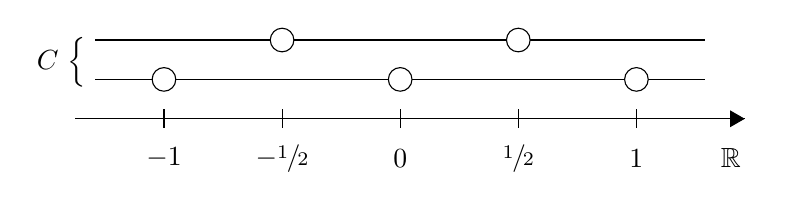
\begin{tikzpicture}
\node (v2) at (4,0.5) {};
\node (v1) at (-4.75,0.5) {};
\draw  (v1) edge (v2);
\draw [-triangle 60] (v1) edge (v2);
\node (v3) at (-4.5,1) {};
\node (v4) at (3.5,1) {};
\draw  (v3) edge (v4);
\node (v5) at (-4.5,1.5) {};
\node (v6) at (3.5,1.5) {};
\draw  (v5) edge (v6);
\draw[fill=white]  (-0.5,1) circle (0.15);
\draw[fill=white]  (-3.5,1) node (v7) {} circle (0.15);
\draw[fill=white]  (2.5,1) circle (0.15);
\draw[fill=white]  (-2,1.5) circle (0.15);
\draw[fill=white]  (1,1.5) circle (0.15);
\draw  (-3.5,0.62) edge (-3.5,0.38);
\draw  (-2,0.62) edge (-2,0.38);
\draw  (-0.5,0.62) edge (-0.5,0.38);
\draw  (2.5,0.62) edge (2.5,0.38);
\draw  (1,0.62) edge (1,0.38);
\node at (-3.5,0) {$-1$};
\node at (-2,0) {$-\sfrac{1}{2}$};
\node at (-0.5,0) {$0$};
\node at (1,0) {$\sfrac{1}{2}$};
\node at (2.5,0) {$1$};
\node at (3.7,0) {$\R$};
\node at (-4.8,1.22) {$C\ \Bigl\{$};
\end{tikzpicture}
\end{figure}

It is clear that removing even one element from $C$ will cause $C$ to fail to be an open cover of $\R$. Therefore, there is no finite subcover of $C$ and hence, $\R$ is not compact.
\ee

\bt
Let $(M,\cO_M)$ and $(N,\cO_N)$ be compact topological spaces. Then $(M\times N,\cO_{M\times N})$ is a compact topological space.
\et

The above theorem easily extends to finite cartesian products. 

\bd
Let $(M,\cO)$ be a topological space and let $C$ be a cover. A \emph{refinement} of $C$ is a cover $R$ such that:
\bse
\forall \, U \in R : \exists \, V \in C : U \se V .
\ese
\ed
Any subcover of a cover is a refinement of that cover, but the converse is not true in general. A refinement $R$ is said to be:
\bit
\item \emph{open} if $R\se \cO$;
\item \emph{locally finite} if for any $p\in M$ there exists a neighbourhood $U(p)$ such that the set:
\bse
\{U \in R \mid U \cap U(p) \neq \vn\}
\ese
is finite as a set.
\eit

Compactness is a very strong property. Hence often times it does not hold, but a weaker and still useful property, called paracompactness, may still hold.

\bd
A topological space $(M,\cO)$ is said to be \emph{paracompact} if every open cover has an open refinement that is locally finite.
\ed

\bc
If a topological space is compact, then it is also paracompact.
\ec

\bd
A topological space $(M,\cO)$ is said to be \emph{metrisable} if there exists a metric $d$ such that the topology induced by $d$ is precisely $\cO$, i.e.\ $\cO_d=\cO$. 
\ed

\bt[Stone]
Every metrisable space is paracompact.
\et




















































































\newpage

\section{Topological manifolds and bundles}

\bd
A paracompact, Hausdorff, topological space $(M,\cO)$ is called a \emph{$d$-dimensional (topological) manifold} if for every point $p\in M$ there exist a neighbourhood $U(p)$ and a homeomorphism 
\ed
\newpage

\section{Differentiable structures: definition and classification}

\subsection{Adding structure by refining the (maximal) atlas}

We saw previously that for a topological manifold $(M,\cO)$, the concept of a $\mathcal{C}^0$-atlas was fully redundant since every atlas is also a $\mathcal{C}^0$-atlas. We will now generalise the notion of a $\mathcal{C}^0$-atlas, or more precisely, the notion of $\mathcal{C}^0$-compatibility of charts, to something which is non-trivial and non-redundant.

\begin{definition}
An atlas $\mathscr{A}$ for a topological manifold is called a {\scalebox{0.75}\FiveFlowerOpen}-\emph{atlas} if any two charts $(U,x), (V,y) \in \mathscr{A}$ are {\scalebox{0.75}\FiveFlowerOpen}-compatible.
\end{definition}

In other words, either $U\cap V = \vn$ or if $U\cap V \neq \vn$, then the transition map $y\circ x^{-1}$ from $x(U\cap V)$ to $y(U\cap V)$ must be {\scalebox{0.75}\FiveFlowerOpen}.
\bse
\begin{tikzcd}
& U\cap V \se M \ar[ldd,"x"'] \ar[rdd,"y"]&\\
&&&\\
x(U\cap V) \se \R^{\dim M} \ar[rr,"y\circ x^{-1}"']& & y(U\cap V)\se \R^{\dim M}
\end{tikzcd}
\ese
Before you think Dr Schuller finally went nuts, the symbol {\scalebox{0.75}\FiveFlowerOpen} is being used as a placeholder for any of the following:
\begin{itemize}
\item ${\scalebox{0.75}\FiveFlowerOpen} = \mathcal{C}^0$: this just reduces to the previous definition;
\item ${\scalebox{0.75}\FiveFlowerOpen} = \mathcal{C}^k$: the transition maps are $k$-times continuously differentiable as maps between open subsets of $\R^{\dim M}$;
\item ${\scalebox{0.75}\FiveFlowerOpen} = \mathcal{C}^\infty$: the transition maps are smooth (infinitely many times differentiable); equivalently, the atlas is $\mathcal{C}^k$ for all $k\geq 0$;
\item ${\scalebox{0.75}\FiveFlowerOpen} = \mathcal{C}^\omega$: the transition maps are (real) analytic, which is stronger than being smooth;
\item ${\scalebox{0.75}\FiveFlowerOpen} =$ complex: if $\dim M$ is even, $M$ is a \emph{complex manifold} if the transition maps are continuous and satisfy the Cauchy-Riemann equations; its complex dimension is $\tfrac{1}{2}\dim M$.
\end{itemize}

As an aside, if you haven't met the Cauchy-Riemann equations yet, recall than since $\R^2$ and $\C$ are isomorphic as sets, we can identify the function 
\bi{rcCl}
f\cl & \R^2 & \to     & \R^2 \\
     &(x,y) & \mapsto & (u(x,y),v(x,y))
\ei
where $u,v \cl \R^2\to\R$, with the function
\bi{rcCl}
f\cl & \C & \to     & \C \\
     &x+\mathrm{i}y & \mapsto & u(x,y)+\mathrm{i}v(x,y).
\ei
If $u$ and $v$ are real differentiable at $(x_0,y_0)$, then $f=u+\mathrm{i}v$ is complex differentiable at $z_0=x_0+\mathrm{i}y_0$ if, and only if, $u$ and $v$ satisfy
\bse
\frac{\partial u}{\partial x}(x_0,y_0)= \frac{\partial v}{\partial y}(x_0,y_0) \quad \land \quad \frac{\partial u}{\partial y}(x_0,y_0)= - \frac{\partial v}{\partial x}(x_0,y_0),
\ese
which are known as the Cauchy-Riemann equations\index{Cauchy-Riemann equations}. Note that differentiability in the complex plane is a much stronger condition than differentiability over the real numbers. If you want to know more, you should take a course in complex analysis or function theory.

We now go back to manifolds.

\begin{theorem}[Whitney] Any maximal $\mathcal{C}^k$-atlas, with $k\geq 1$, contains a $\mathcal{C}^\infty$-atlas. Moreover, any two maximal $\mathcal{C}^k$-atlases that contain the same $\mathcal{C}^\infty$-atlas are identical.
\end{theorem}

An immediate implication is that if we can find a $\mathcal{C}^1$-atlas for a manifold, then we can also assume the existence of a $\mathcal{C}^\infty$-atlas for that manifold. This is not the case for topological manifolds in general: a space with a $\mathcal{C}^0$-atlas may not admit any $\mathcal{C}^1$-atlas. But if we have at least a $\mathcal{C}^1$-atlas, then we can obtain a $\mathcal{C}^\infty$-atlas simply by removing charts, keeping only the ones which are $\mathcal{C}^\infty$-compatible.

Hence, for the purposes of this course, we will not distinguish between $\mathcal{C}^k$ ($k\geq 1$) and $\mathcal{C}^\infty$-manifolds in the above sense.

We now give the explicit definition of a $\mathcal{C}^k$-manifold.

\bd
A $\mathcal{C}^k$\emph{-manifold}\index{manifold} is a triple $(M,\cO,\mathscr{A})$, where $(M,\cO)$ is a topological manifold and $\mathscr{A}$ is a maximal $\mathcal{C}^k$-atlas.
\ed

\br 
A given topological manifold can carry different incompatible atlases.
\er

Note that while we only defined compatibility of charts, it should be clear what it means for two atlases of the same type to be compatible.

\bd
Two {\scalebox{0.75}\FiveFlowerOpen}-atlases $\mathscr{A}$, $\mathscr{B}$ are \emph{compatible}\index{atlas!compatible} if their union $\mathscr{A}\cup\mathscr{B}$ is again a {\scalebox{0.75}\FiveFlowerOpen}-atlas, and are incompatible otherwise.
\ed

Alternatively, we can define the compatibility of two atlases in terms of the compatibility of any pair of charts, one from each atlas.

\be
Let $(M,\cO)=(\R,\cO_\mathrm{std})$. Consider the two atlases $\mathscr{A}=\{(\R,\id_\R)\}$ and $\mathscr{B}=\{(\R,x)\}$, where $x\cl a \mapsto \sqrt[3]{a}$. Since they both contain a single chart, the compatibility condition on the transition maps is easily seen to hold (in both cases, the only transition map is $\id_\R$). Hence they are both $\mathcal{C}^\infty$-atlases.

Consider now $\mathscr{A}\cup\mathscr{B}$. The transition map $\id_\R\circ x^{-1}$ is the map $a\mapsto a^3$, which is smooth. However, the other transition map, $x\circ\id_\R^{-1}$, is the map $x$, which is not even differentiable once (the first derivative at $0$ does not exist). Consequently, $\mathscr{A}$ and $\mathscr{B}$ are not even $\mathcal{C}^1$-compatible.
\ee

The previous example shows that we can equip the real line with (at least) two different incompatible $\mathcal{C}^\infty$-structures. This looks like a disaster as it implies that there is an arbitrary choice to be made about which differentiable structure to use. Fortunately, the situation is not as bad as it looks, as we will see in the next sections.

\subsection{Differentiable manifolds}
\index{manifold!differentiable}
\bd
Let $\phi\cl M\to N$ be a map, where $(M,\cO_M,\mathscr{A}_M)$ and $(N,\cO_N,\mathscr{A}_N)$ are $\mathcal{C}^k$-manifolds. Then $\phi$ is said to be ($\mathcal{C}^k$-)\emph{differentiable at} $p\in M$ if for some charts $(U,x)\in\mathscr{A}_M$ with $p\in U$ and $(V,y)\in\mathscr{A}_N$ with $\phi(p)\in V$, the map $y\circ\phi\circ x^{-1}$ is $k$-times continuously differentiable at $x(p)\in x(U)\se\R^{\dim M}$ in the usual sense.
\bse
\begin{tikzcd}
U\se M \ar[rr,"\phi"] \ar[dd,"x"] && V\se N \ar[dd,"y"]\\
&&\\
x(U)\se\R^{\dim M}\ar[rr,"y\circ\phi\circ x^{-1}"] && y(V)\se\R^{\dim N}
\end{tikzcd}
\ese
\ed
The above diagram shows a typical theme with manifolds. We have a map $\phi\cl M\to N$ and we want to define some property of $\phi$ at $p\in M$ analogous to some property of maps between subsets of $\R^d$. What we typically do is consider some charts $(U,x)$ and $(V,y)$ as above and define the desired property of $\phi$ at $p\in U$ in terms of the corresponding property of the downstairs map $y\circ\phi\circ x^{-1}$ at the point $x(p)\in\R^d$.

Notice that in the previous definition we only require that \emph{some} charts from the two atlases satisfy the stated property. So we should worry about whether this definition depends on which charts we pick. In fact, this ``lifting'' of the notion of differentiability from the chart representation of $\phi$ to the manifold level is well-defined.

\bp
The definition of differentiability is well-defined.
\ep

\bq
We want to show that if $y\circ\phi\circ x^{-1}$ is differentiable at $x(p)$ for some $(U,x)\in\mathscr{A}_M$ with $p\in U$ and $(V,y)\in\mathscr{A}_N$ with $\phi(p)\in V$, then $\widetilde y\circ\phi\circ \widetilde x^{-1}$ is differentiable at $\widetilde x(p)$ for all charts $(\widetilde U,\widetilde x)\in\mathscr{A}_M$ with $p\in \widetilde U$ and $(\widetilde V,\widetilde y)\in\mathscr{A}_N$ with $\phi(p)\in \widetilde V$.
\bse
\begin{tikzcd}
\widetilde x(U\cap\widetilde U)\se\R^{\dim M}\ar[rr,"\widetilde y\circ\phi\circ \widetilde x^{-1}"] && \widetilde y(V\cap\widetilde V)\se\R^{\dim N}\\
&&\\
U\cap\widetilde U\se M \ar[rr,"\phi"] \ar[dd,"x"] \ar[uu,"\widetilde x"'] && V\cap\widetilde V\se N \ar[dd,"y"] \ar[uu,"\widetilde y"']\\
&&\\
x(U\cap\widetilde U)\se\R^{\dim M}\ar[rr,"y\circ\phi\circ x^{-1}"] \ar[uuuu,bend left=70,"\widetilde x\circ x^{-1}"]&& y(V\cap\widetilde V)\se\R^{\dim N} \ar[uuuu,bend right=70,"\widetilde y\circ y^{-1}"']
\end{tikzcd}
\ese
Consider the map $\widetilde x\circ x^{-1}$ in the diagram above. Since the charts $(U,x)$ and $(\widetilde U,\widetilde x)$ belong to the same $\mathcal{C}^k$-atlas $\mathscr{A}_M$, by definition the transition map $\widetilde x\circ x^{-1}$ is $\mathcal{C}^k$-differentiable as a map between subsets of $\R^{\dim M}$, and similarly for $\widetilde y\circ y^{-1}$. We now notice that we can write:
\bse
\widetilde y\circ\phi\circ \widetilde x^{-1} = (\widetilde y\circ y^{-1})\circ(y\circ\phi\circ x^{-1})\circ(\widetilde x\circ x^{-1})^{-1}
\ese
and since the composition of $\mathcal{C}^k$ maps is still $\mathcal{C}^k$, we are done.
\eq
This proof shows the significance of restricting to $\mathcal{C}^k$-atlases. Such atlases only contain charts for which the transition maps are $\mathcal{C}^k$, which is what makes our definition of differentiability of maps between manifolds well-defined.

The same definition and proof work for smooth ($\mathcal{C}^\infty$) manifolds, in which case we talk about \emph{smooth maps}. As we said before, this is the case we will be most interested in.

\be
Consider the smooth manifolds $(\R^d,\cO_\mathrm{std},\mathscr{A}_d)$ and $(\R^{d'},\cO_\mathrm{std},\mathscr{A}_{_d'})$, where $\mathscr{A}_d)$ and $\mathscr{A}_{_d'})$ are the maximal atlases containing the charts $(\R^d,\id_{\R^d})$ and $(\R^{d'},\id_{\R^{d'}})$ respectively, and let $f\cl \R^{d}\to \R^{d'}$ be a map. The diagram defining the differentiability of $f$ with respect to these charts is
\bse
\begin{tikzcd}
\R^{d} \ar[rrrr,"f"] \ar[dd,"\id_{\R^d}"] &&&& \R^{d'} \ar[dd,"\id_{\R^{d'}}"]\\
&&\\
\R^{d} \ar[rrrr,"\id_{\R^{d'}}\circ f\circ (\id_{\R^d})^{-1}"]&&&& \R^{d'}
\end{tikzcd}
\ese
and, by definition, the map $f$ is smooth as a map between manifolds if, and only if, the map $\id_{\R^{d'}}\circ f\circ (\id_{\R^d})^{-1}=f$ is smooth in the usual sense.
\ee

\be
Let $(M,\cO,\mathscr{A})$ be a $d$-dimensional smooth manifold and let $(U,x)\in\mathscr{A}$. Then $x\cl U \to x(U)\se \R^d$ is smooth. Indeed, we have
\bse
\begin{tikzcd}
U \ar[rrr,"x"] \ar[dd,"x"] &&& x(U) \ar[dd,"\id_{x(U)}"]\\
&&\\
x(U)\se\R^{d} \ar[rrr,"\id_{x(U)}\circ x\circ x^{-1}"]&&& x(U)\se\R^{d} 
\end{tikzcd}
\ese
Hence $x\cl U \to x(U)$ is smooth if, and only if, the map $\id_{x(U)}\circ x\circ x^{-1}=\id_{x(U)}$ is smooth in the usual sense, which it certainly is.

The coordinate maps $x^i:={\proj_i}\circ x\cl U \to \R$ are also smooth. Indeed, consider the diagram
\bse
\begin{tikzcd}
U \ar[rrr,"x^i"] \ar[dd,"x"] &&& \R \ar[dd,"\id_\R"]\\
&&\\
x(U)\se\R^{d} \ar[rrr,"{\id_\R}\circ x^i\circ x^{-1}"]&&& \R 
\end{tikzcd}
\ese
Then, $x^i$ is smooth if, and only if, the map
\bse
{\id_\R}\circ x^i\circ x^{-1} =  x^i\circ x^{-1} = \proj_i
\ese
is smooth in the usual sense, which it certainly is.
\ee

\subsection{Classification of differentiable structures}

\bd
Let $\phi\cl M \to N$ be a bijective map between smooth manifolds. If both $\phi$ and $\phi^{-1}$ are smooth, then $\phi$ is said to be a \emph{diffeomorphism}\index{diffeomorphism}\index{isomorphism!of smooth manifolds}.
\ed

Diffeomorphisms are the structure preserving maps between smooth manifolds. 

\bd
Two manifolds $(M,\cO_M,\mathscr{A}_M)$, $(N,\cO_N,\mathscr{A}_N)$ are said to be \emph{diffeomorphic} if there exists a diffeomorphism $\phi\cl M\to N$ between them. We write $M \cong_\text{diff}N$.
\ed

Note that if the differentiable structure is understood (or irrelevant), we typically write $M$ instead of the triple $(M,\cO_M,\mathscr{A}_M)$.

\br
Being diffeomorphic is an equivalence relation. In fact, it is customary to consider diffeomorphic manifolds to be \emph{the same} from the point of view of differential geometry. This is similar to the situation with topological spaces, where we consider homeomorphic spaces to be the same from the point of view of topology. This is typical of all structure preserving maps.
\er

Armed with the notion of diffeomorphism, we can now ask the following question: how many smooth structures on a given topological space are there, up to diffeomorphism?

The answer is quite surprising: it depends on the dimension of the manifold!

\begin{theorem}[Radon-Moise]
Let $M$ be a manifold with $\dim M = 1, 2$, or $3$. Then there is a unique smooth structure on $M$ up to diffeomorphism.
\end{theorem}

Recall that in a previous example, we showed that we can equip $(\R,\cO_\mathrm{std})$ with two incompatible atlases $\mathscr{A}$ and $\mathscr{B}$. Let $\mathscr{A}_\mathrm{max}$ and $\mathscr{B}_\mathrm{max}$ be their extensions to maximal atlases, and consider the smooth manifolds $(\R,\cO_\mathrm{std},\mathscr{A}_\mathrm{max})$ and  $(\R,\cO_\mathrm{std},\mathscr{B}_\mathrm{max})$. Clearly, these are different manifolds, because the atlases are different, but since $\dim \R=1$, they must be diffeomorphic.

The answer to the case $\dim M > 4$ (we emphasize $\dim M \neq 4$) is provided by \emph{surgery theory}. This is a collection of tools and techniques in topology with which one obtains a new manifold from given ones by performing surgery on them, i.e.\ by cutting, replacing and gluing parts in such a way as to control topological invariants like the fundamental group. The idea is to understand all manifolds in dimensions higher than 4 by performing surgery systematically. In particular, using  surgery theory, it has been shown that there are only finitely many smooth manifolds (up to diffeomorphism) one can make from a topological manifold.

This is not as neat as the previous case, but since there are only finitely many structures, we can still enumerate them, i.e.\ we can write an exhaustive list.

While finding all the differentiable structures may be difficult for any given manifold, this theorem has an immediate impact on a physical theory that models spacetime as a manifold. For instance, some physicists believe that spacetime should be modelled as a $10$-dimensional manifold (we are neither proposing nor condemning this view). If that is indeed the case, we need to worry about which differentiable structure we equip our 10-dimensional manifold with, as each different choice will likely lead to different predictions. But since there are only finitely many such structures, physicists can, at least in principle, devise and perform finitely many experiments to distinguish between them and determine which is the right one, if any.

We now turn to the special case $\dim M = 4$. The result is that if $M$ is a non-compact topological manifold, then there are uncountably many non-diffeomorphic smooth structures that we can equip $M$ with. In particular, this applies to $(\R^4,\cO_\mathrm{std})$.

In the compact case there are only partial results. By way of example, here is one such result.

\bp
If $(M,\cO)$, with $\dim M = 4$, has $b_2>18$, where $b_2$ is the second Betti number, then there are countably many non-diffeomorphic smooth structures that we can equip $(M,\cO)$ with. 
\ep

Betti numbers are defined in terms of homology groups, but intuitively we have:
\begin{itemize}
\item $b_0$ is the number of connected components a space has;
\item $b_1$ is the number of circular (1-dimensional) holes a space has;
\item $b_2$ is the number of 2-dimensional holes a space has;
\end{itemize}
and so on. Hence if a manifold has a number of 2-dimensional holes greater than 18, then there only countably many structures that we can choose from, but they are still infinitely many.












\newpage

\section{Tensor space theory I: over a field}



\section{Differential structures: the pivotal concept of tangent vector spaces}



\section{Construction of the tangent bundle}



\section{Tensor space theory II: over a ring}



\section{Grassmann algebra and de Rham cohomology}



\section{Lie groups and their Lie algebras}



\section{Classification of Lie algebras and Dynkin diagrams}



\section{The Lie group $SL(2,\C)$ and its Lie algebra $\mathfrak{sl}(2,\C)$}



\section{Dynkin diagrams from Lie algebras, and vice versa}



\section{Representation theory of Lie groups and Lie algebras}



\section{Reconstruction of a Lie group from its algebra}



\section{Principal fibre bundles}



\section{Associated fibre bundles}



\section{Connections and connection 1-forms}



\section{Local representations of a connection on the base manifold: Yang-Mills fields}



\section{Parallel transport}



\section{Curvature and torsion on principal bundles}



\section{Covariant derivatives}



\section{Application: Quantum mechanics on curved spaces}



\section{Application: Spin structures}



\section{Application: Kinematical and dynamical symmetries}



%----------------------------------------------------------------------------------------
%	BIBLIOGRAPHY
%----------------------------------------------------------------------------------------

%\renewcommand{\refname}{\spacedlowsmallcaps{References}} % For modifying the bibliography heading

%\bibliographystyle{unsrt}

%\bibliography{sample.bib} % The file containing the bibliography

%----------------------------------------------------------------------------------------

\end{document}